\documentclass[conference]{IEEEtran}
\IEEEoverridecommandlockouts
% The preceding line is only needed to identify funding in the first footnote. If that is unneeded, please comment it out.
\usepackage{cite}
\usepackage{amsmath,amssymb,amsfonts}
\usepackage{algorithmic}
\usepackage{graphicx}
\usepackage{textcomp}
\usepackage{xcolor}
\usepackage[export]{adjustbox}
\def\BibTeX{{\rm B\kern-.05em{\sc i\kern-.025em b}\kern-.08em
    T\kern-.1667em\lower.7ex\hbox{E}\kern-.125emX}}
\usepackage{algorithm}
\usepackage{algorithmic}
\usepackage{listings}
\setlength{\marginparwidth}{3cm}
\usepackage{subcaption}
\usepackage{enumitem}

\usepackage[colorinlistoftodos]{todonotes} %add disable in the params to remove all todos
%commands for todos
\newcommand{\Todo}[1]{\todo[inline, color=red!40]{#1}}
\newcommand{\Fixme}[1]{\todo[inline, color=orange!40]{#1}}
\newcommand{\Comment}[1]{\todo[inline, color=green!40]{#1}}
\newcommand{\alphaz}{\textsc{\texttt{AlphaZ}}}
\newcommand{\alfa}{\textsc{\texttt{Alpha}}}
\newcommand{\squeezeup}{\vspace{-2.5mm}}



% remove it:start???
\usepackage{xcolor}


\newsavebox\MBox
\newcommand\Cline[2][red]{{\sbox\MBox{$#2$}%
  \rlap{\usebox\MBox}\color{#1}\rule[-1.2\dp\MBox]{\wd\MBox}{0.5pt}}}
  
  
 \lstset{ 
  backgroundcolor=\color{white},   % choose the background color; you must add \usepackage{color} or \usepackage{xcolor}; should come as last argument
  %basicstyle=\footnotesize,        % the size of the fonts that are used for the code
  basicstyle=\scriptsize,        % the size of the fonts that are used for the code
  breakatwhitespace=false,         % sets if automatic breaks should only happen at whitespace
  breaklines=true,                 % sets automatic line breaking
  captionpos=b,                    % sets the caption-position to bottom
  commentstyle=\color{mygreen},    % comment style
  deletekeywords={...},            % if you want to delete keywords from the given language
  escapeinside={\%*}{*)},          % if you want to add LaTeX within your code
  extendedchars=true,              % lets you use non-ASCII characters; for 8-bits encodings only, does not work with UTF-8
  firstnumber=1,                % start line enumeration with line 1000
  frame=single,	                   % adds a frame around the code
  keepspaces=true,                 % keeps spaces in text, useful for keeping indentation of code (possibly needs columns=flexible)
  keywordstyle=\color{blue},       % keyword style
  language=Octave,                 % the language of the code
  morekeywords={*,...},            % if you want to add more keywords to the set
  numbers=left,                    % where to put the line-numbers; possible values are (none, left, right)
  numbersep=-8pt,                   % how far the line-numbers are from the code
  numberstyle=\tiny, % the style that is used for the line-numbers
  rulecolor=\color{black},         % if not set, the frame-color may be changed on line-breaks within not-black text (e.g. comments (green here))
  showspaces=false,                % show spaces everywhere adding particular underscores; it overrides 'showstringspaces'
  showstringspaces=false,          % underline spaces within strings only
  showtabs=false,                  % show tabs within strings adding particular underscores
  stepnumber=1,                    % the step between two line-numbers. If it's 1, each line will be numbered
  stringstyle=\color{mymauve},     % string literal style
  tabsize=2,	                   % sets default tabsize to 2 spaces
  title=\lstname                   % show the filename of files included with \lstinputlisting; also try caption instead of title
  xleftmargin=-5pt,
  framexleftmargin=-5pt,
  framexrightmargin=-2pt,
  framexbottommargin=0pt,
  framextopmargin=0pt,
}
\newcommand*{\colorboxed}{}
\def\colorboxed#1#{%
  \colorboxedAux{#1}%
}
\newcommand*{\colorboxedAux}[3]{%
  % #1: optional argument for color model
  % #2: color specification
  % #3: formula
  \begingroup
    \colorlet{cb@saved}{.}%
    \color#1{#2}%
    \boxed{%
      \color{cb@saved}%
      #3%
    }%
  \endgroup
}
% remove it:end???    
\begin{document}

\title{Accelerating the BPMax Algorithm for RNA-RNA Interaction}

\author{\IEEEauthorblockN{Chiranjeb Mondal}
\IEEEauthorblockA{\textit{Department of Computer Science} \\
\textit{Colorado State University}\\
Fort Collins, CO, USA \\
chiranjeb.mondal@colostate.edu}
\and
\IEEEauthorblockN{Sanjay Rajopadhye}
\IEEEauthorblockA{\textit{Department of Computer Science} \\
\textit{Colorado State University}\\
Fort Collins, CO, USA \\
sanjay.rajopadhye@colostate.edu}
}
\maketitle
\begin{abstract}
RNA-RNA interactions (RRI) play an important role in various biological processes such as gene transcription, and are known to play a critical role in diseases such as cancer and Alzheimer’s, necessitating efficient computational tools. To date, RRI programs like BPMax were developed and optimized by hand, and this is prone to human error, and costly to develop and maintain.  Its high complexity ($\Theta(N^3M^3)$ in time and $\Theta(N^2M^2)$ in space) make it both essential and a challenge to parallelize it.   In this paper, we present a parallelization of BPMax on a single shared memory CPU platform.  From a mathematical specification of the dynamic programming algorithm, we generate highly optimized code that achieves over $100\times$ speedup over the baseline program employing a standard ``diagonal-by-diagonal'' execution order. We achieve 76~GFLOPS, which is about a fifth of our platform's peak theoretical single-precision performance for max-plus computation. The main kernel in the algorithm whose complexity is $\Theta(N^3M^3)$ attains 117~GFPLOS. We do this with a polyhedral code generation tool, \alphaz, that takes user-specified mapping directives and automatically generates optimized C code that enhances parallelism and locality.
\alphaz\ allows the user to explore various schedules, memory-maps, and parallelization approaches, as well as tiling of the most dominant part of the computation.


%We make  handwritten C code related to the actual algorithm, except a few compiler directives and minor optimizations of variable initialization.  
%Besides overall speedup, our focus was to optimize the most compute-intensive part of the BPMax program which has complexity of $O(M^3N^3)$.  Our optimization speeds up this portion of the computation by 170x over the base version which is a sequential improvement between $1.4\times$ to $2\times$ over a similar type of kernel optimized previously using polyhedral acceleration on moderate size input sequences.

\end{abstract}

\begin{IEEEkeywords}
RRI, BPMax, polyhedral model, tiling
\end{IEEEkeywords}
%\todo{Test}
\section{\uppercase{Introduction}}
Ribonucleic acid (RNA) is the origin of life. It plays an essential role in the coding, decoding, regulation, and expression of genes. RNA is a single strand formed by a sequence of four different types of nucleotides – Adenine (A), Uracil (U), Guanine (G), and Cytosine (C), which form a repeating structure.  Different nucleotides may form bonds of varying strength. A single RNA strand folds into itself. Also, two different RNA strands can interact with each other, resulting in the secondary structure, which can provide valuable  information about a biological function.
%Guanine forms the strongest bond with Cytosine, Adenine forms the next strongest bond with Uracil, and Uracil forms the weakest bond with Guanine. 
%A single RNA strand folds into itself. Also, two different RNA strands can interact with each other, resulting in the secondary structure. Knowledge of such structure can provide useful information about a biological function and may be used in experiments. 

% Please refer to  ~\cite{Mortimer_2014}, ~\cite{Ledda2018} for more information.


%\Todo{Please take care of the warnings.  They are because you did a cut and paste of your equations, and the subtraction operator is not the usual - but an extend-dash.  You may comment out todo notes that have been resolved, Like I have for the claims in the abstract.}

%Researchers have long been studying these interactions and proposed different interaction models.  One of the early studies on interactions between nucleotides of single RNA was proposed by Nussinov in 1978 that predicts secondary structure\cite{Nussinov1978}. RNA-RNA interactions have been moved to spotlight in biology since mid 1990s with significant RNA interference discovery. 
Researchers have long been studying these interactions and proposed different models. In 1978, Nussinov presented a model \cite{Nussinov1978} that predicts secondary structure from single RNA folding. RNA-RNA interactions have been moved to the spotlight in biology since the mid-1990s with significant RNA interference discovery. Chitsaz et al.\cite{Chitsaz2009} developed piRNA - one of the most comprehensive thermodynamic models for RRI.  It has an $\Theta(N^4M^2+N^2M^4)$  time and $\Theta(N^4+M^4)$ space complexity, %where $M$ and $N$ is the number of nucleotides present in each RNA sequence.
for sequences of length $M$ and $N$. It uses $96$ dynamic tables.  However, running this compute and memory intensive program is extremely challenging. It takes days and months to get experimental results. So, Ebrahimpour-Boroojeny et al. \cite{EbrahimpourBoroojeny2019}  retreated from the slow comprehensive model and developed the BPPart for base-pair partition and BPMax for base-pair maximization. They use a simplified energy model and consider only base pair counting. Both of them have similar asymptotic time and space complexity of $\Theta(M^3N^3)$  and $\Theta(M^2N^2)$. BPPart uses $11$ tables, and BPMax uses a single one.  Nevertheless, the original implementation of even BPMax suffers from poor performance as the input size grows.

Ebrahimpour-Boroojeny et al. conclude that BPMax \cite{EbrahimpourBoroojeny2019} captures a significant portion of the thermodynamic information. The Pearson and Spearman’s rank correlation between piRNA and BPMax is  $0.904$ at $-180$\textdegree\textit{C} and  $0.836$  at 37\textdegree\textit{C} highlighting its importance.  BPMax and other RRI algorithms such as piRNA~\cite{Chitsaz2009}, IRIS~\cite{Pervouchine2004IRISIR}, RIP~\cite{Huang2009} follow similar recurrence patterns. So, besides the practical usefulness of BPMax, the learning and insights gleaned from this optimization approach can be applied to the other RRI interaction algorithms with similar recurrence patterns.


Performance optimization requires exploiting parallelism and locality at multiple levels. It is a difficult task and often leads to hand-crafted code. Manual optimization is neither easily portable (e.g., to different platforms where different kinds of optimization are needed) nor easily maintainable (e.g., changing the optimization strategy may require changes to many parts of the code). This challenge grows as the complexity of the program increases. It is highly desirable that the highly optimized programs get generated from a simple correct program together with a set of performance tuning hints or directives.

Fortunately, RRI algorithms fit the requirements of the \emph{polyhedral model}~\cite{sanjay-fst-tcs, quinton-jvsp89, feautrier91, feautrier92a, feautrier92b}  - a mathematical formalism that allows for just such program transformations.  The polyhedral compilation has been the subject of intense research for 35~years, and yet, even a state-of-the-art polyhedral tool like PLUTO~\cite{Bondhugula2015PLuToAP, Bondhugula2008} does not yield satisfactory performance~\cite{Varadarajan2016}. Many of the performance optimization strategies need some careful thought by an expert.  This gap can be bridged by a tool that allows semi-automatic transformation like Chill~\cite{Chen08chill:a}. At CSU, we are developing and working with a similar tool, \alphaz~\cite{sanjay-lcpc2012}, that operates at a higher level of abstraction.
%\noindent
%\begin{itemize}[wide, nosep, labelindent = 0pt, topsep = 1ex]
\begin{itemize}[wide, nosep, labelindent = 0pt]
\item [The paper makes the following contributions:]
%\item This is the first time a complex RRI program like BPMax has been optimized using a polyhedral compilation framework such as \alphaz\ in its entirety. It is also the first attempt to optimize BPMax on the CPU.
\item This is the first time a complex RRI program like BPMax has been optimized using \alphaz\ in its entirety. Previous attempts were limited to a micro-kernel only. It is also the first attempt to optimize BPMax on the CPU.
\item We generate highly optimized code for BPMax using polyhedral transformations that achieves over $100\times$ speedup over the original program shown in Figure~\ref{fig:bpm_quick_compare}. The most compute-intensive part of the BPMax achieves a $170\times$ speedup over the original implementation, a  $1.5\times$ - $2\times$ improvement over a similar kernel optimized previously. 
\item The compilation scripts and optimized version of the BPMax program are available in GitHub public repository ~\cite{MondalBPMax}.
\end{itemize}

\begin{figure}[htbp]
\centering
\begin{subfigure}[htbp]{0.49\linewidth}
\centering
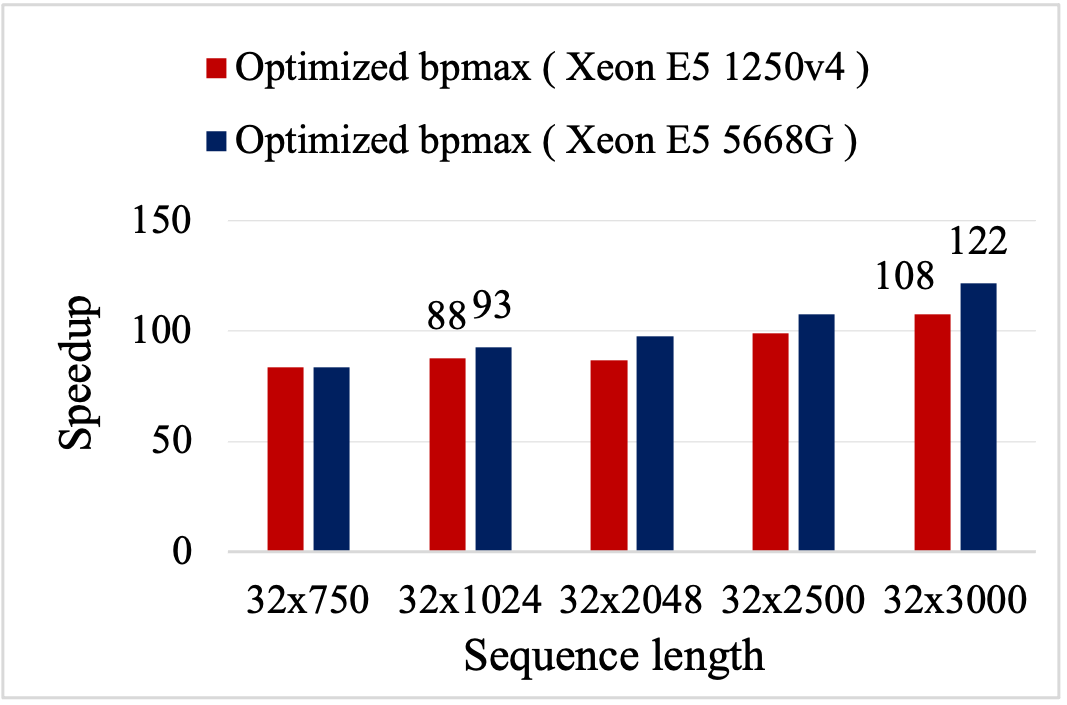
\includegraphics[scale=0.52, trim=4 4 4 4,clip]{figure_highlight_speed_up2.png}
\caption{Speedup over base program}
\label{fig:quick_speedup}
\end{subfigure}
\begin{subfigure}[htbp]{0.49\linewidth}
\centering
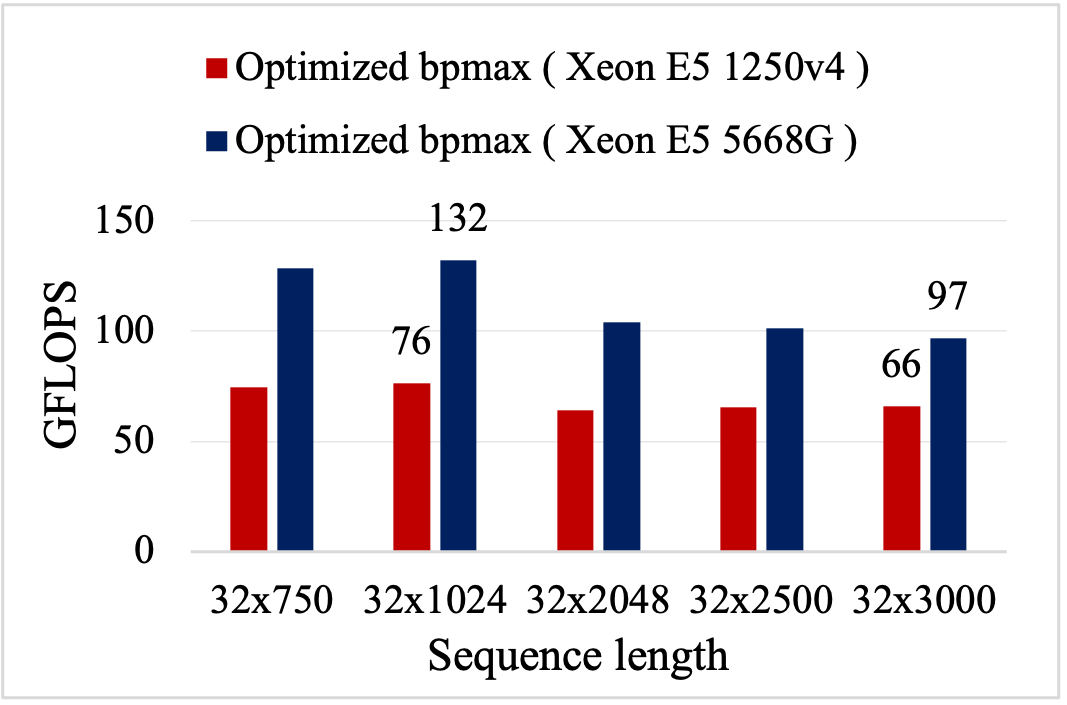
\includegraphics[scale=0.52, trim=4 4 4 4,clip]{figure_highlight_perf2.png}
\caption{Single-precision performance}
\label{fig:quick_performance}
\end{subfigure}
\caption{Summary of the optimization results}
\label{fig:bpm_quick_compare}
\end{figure}

The paper proceeds as follows. We first set up the context and background of our work to highlight the BPMax algorithm, discuss the polyhedral model's role, and application of \alphaz\ . Then, we discuss multiple phases of the optimization process, the rationale behind different schedules, processor allocations, and memory mappings. Finally, we go over our performance results and conclude the paper with challenges and future directions.

\section{\uppercase{Related Work}}
%One of the early studies on interactions between nucleotides of single RNA was proposed by Nussinov in 1978 that predicts secondary structure\cite{Nussinov1978}. Palkowski et al. \cite{Palkowski2019} have used the polyhedral model to optimize this algorithm.
%This algorithm computes a structure based on the probability that maximizes the number of base-pairs. This has a complexity of $\Theta(N^3)$ time and $\Theta(N^2)$ space. 
%Later new algorithms got introduced to improve the energy model. Most of these algorithms use base pair maximization (BPM). 
%Work was done to optimize and parallelize these algorithms on CPU platform. 
% Li et al. has worked on CPU and GPU version of BPM \cite{Li2013} to improve its performance. Swenson et al. \cite{Swenson2012}  worked on a parallel secondary structure prediction program for multi-core desktop. However, all these effort were related to single RNA strand folding.

There was no previous example of significant success of RRI optimization using polyhedral compilation to the best of our knowledge.  Palkowski et al. \cite{Palkowski2019} have used the polyhedral model to optimize Nussinov's algorithm ~\cite{Nussinov1978}. However, it is related to single RNA strand folding only.

Varadrajan~\cite{Varadarajan2016, Varadarajan2019} applied semi-automatic transformation using \alphaz\ for a simplified surrogate mini-app that mimicked the dependence pattern to focus only on the most compute-intensive portion of the original piRNA. The original shared-memory OpenMP programs related to BPMax, BPPart, and piRNA try to achieve maximum parallelization without auto-vectorization and suffer very poor locality. She exploited locality using both coarse and fine-grain parallelism and achieved around $100 \times$ speedup.  

Glidemaster\cite{Gildemaster2020} achieved significant speedup on a windowed version of the BPMax on GPU. However, only up to a limited number of nucleotide sequences or a window of nucleotide sequences can be processed on GPU due to memory constraints. Also, the cost of moving data out of the GPU memory negatively impacts the overall performance. So, it is crucial to speedup the algorithm on the CPU to avoid these constraints. It can also further open up the possibility of a higher degree of parallelism over multiple machines.
\section{\uppercase{Background}}
This section highlights the BPMax algorithm, summarizes the polyhedral model, and then describes the code-generation technique using \alphaz\ .

\subsection{\uppercase{BPMax ALGORITHM}}
BPMax uses weighted base-pair counting for base-pair maximization. It considers  both intermolecular and intramolecular
\begin{figure}[htbp]
\centerline{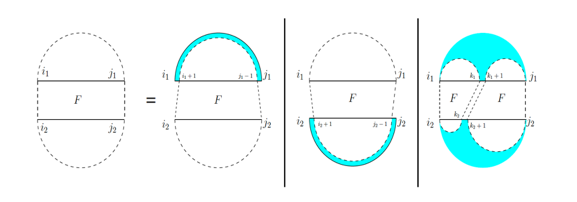
\includegraphics[scale=.9]{bpmax.png}}
\caption{The four cases defining table $F$}
\label{fig:bpm_eddy_rivas}
\end{figure}
\begin{equation}
\label{eqn:bpm_recurrence}
F_{i_{1},j_{1}, i_{2}, j_{2}}  =max \left \{\begin{array}{lr}
                 S_{i_{2}, j_{2}}^{(2)}   \hspace{10pt} j_{1}\le i_{1} \\
                 \\
                 S_{i_{1}, j_{1}}^{(1)}   \hspace{10pt} j_{2}\le i_{2} \\
                 \\
                 \text{iscore}(i_{1}, i_{2})   \hspace{20pt}  i_{1} = j_{1} \text{ and }  i_{2} = j_{2} \\
                 \\
                 \max[ \colorboxed{brown}{F_{i_{1}+1, j_{1}-1, i_{2}, j_{2}}} + \text{score}(i_{1}, j_{1}), \\
                      \colorboxed{gray}{F_{i_{1}, j_{1}, i_{2}+1, j_{2}-1}} + \text{score}(i_{2}, j_{2}), \\
                      H_{i_{1},j_{1},i_{2},j_{2}}]   \hspace{30pt}  otherwise
               \end{array}
           \right. \\
\end{equation}
\begin{equation}
\label{eqn:bpm_recurrence_h}
H_{i_{1},j_{1},i_{2},j_{2}} \\ = \max \left \{\begin{array}{lr}
                 S^{(1)}(i_{1}, j_{1})  + S^{(2)}(i_{2}, j_{2}), \\
                 \\
                \\D_{i_{1},j_{1},i_{2},j_{2}}\\
                 \\
                 \colorboxed{green}{\max\limits_{k_{2}=i_{2}}^{j_{2}-1} S^{(2)}(i_{2}, k_{2}) + F_{i_{1},j_{1}, k_{2}+1, j_{2}}}\\
                 \\
                 \colorboxed{orange}{{\max\limits_{k_{2}=i_{2}}^{j_{2}-1} F_{i_{1},j_{1}, i_{2}, k_{2}} + S^{(2)}(k_{2}+1, j_{2})}}\\
                 \\
                 \colorboxed{violet}{\max\limits_{k_{1}=i_{1}}^{j_{1}-1}  S^{(1)}(i_{1}, k_{1}) + F_{k_{1}+1,j_{1},i_{2}, j_{2}}}\\
                 \\
                 \colorboxed{yellow}{\max\limits_{k_{1}=i_{1}}^{j_{1}-1} F_{i_{1},k_{1}, i_{2}, j_{2}}+ S^{(1)}(k_{1}+1, j{1})} \\
               \end{array}
           \right. \\
\end{equation}
\begin{equation}
\label{eqn:bpm_recurrence_h_dmaxp1}
D_{i_{1},j_{1},i_{2},j_{2}} \\ = 
                 \colorboxed{blue}{\max\limits_{k_{1}=i_{1}}^{j_{1}-1} \max\limits_{k_{2}=i_{2}}^{j_{2}-1} F_{i_{1},k_{1}, i_{2}, k_{2}}+ F_{k_{1}+1,j_{1}, k_{2}+1, j_{2}}}\\
\end{equation}
base pairings. It does not allow pseudo-knots or crossings. Mathematically, it produces a four-dimensional triangular table - $F$-table (a triangular collection of triangles) based on two input sequences. Figure~\ref{fig:bpm_eddy_rivas} shows the main cases for the $F$-table using Eddy-Rivas diagram. Equation~\ref{eqn:bpm_recurrence},   Equation~\ref{eqn:bpm_recurrence_h}, and Equation~\ref{eqn:bpm_recurrence_h_dmaxp1} show the complete recurrence equation of BPMax. Equation~\ref{eqn:bpm_recurrence_h_dmaxp1} highlighted in the blue color represents the double max-plus operation. It is the most compute-intensive portion of the algorithm. We use the same colors to highlight the dependence pattern in section \ref{section:methods}.


\subsection{Polyhedral Model}
The Polyhedral model~\cite{sanjay-fst-tcs, quinton-jvsp89, feautrier91, feautrier92a, feautrier92b} is a mathematical framework for automatic optimization and parallelization of affine programs. A polyhedron is the intersection of finitely many half-spaces. It can be bounded (polytope) or unbounded. Static control parts like variables, iteration space (loop nests), and dependencies can be represented using polyhedra. 
\begin{lstlisting}[label={listing:scan}, language=Caml, caption={Prefix sum}]
    for(int i=0;i<7;i++ ) {
        sum[i]=0;
        for (int j=0 ; j<=i;  j++) 
            sum[i] += array[j]; 
    }
\end{lstlisting}
Let us consider the prefix sum code highlighted in Listing~\ref{listing:scan}   that computes the prefix-sum of an array of size $7$. The iteration space for this computation can be represented using the intersection of the finite half-spaces or set of inequalities such as $j \leq i$,  $i \leq 6$  and $j = 0$ .  The points in the iteration spaces are marked with the dots represented by the polyhedron with vertices - $(0, 0), (0, 6)$, and $(6, 0)$.
\begin{figure}[htbp]
\begin{adjustbox}{varwidth=\textwidth,margin=0 {\abovecaptionskip} 0 0, frame=0.00pt}
\centerline{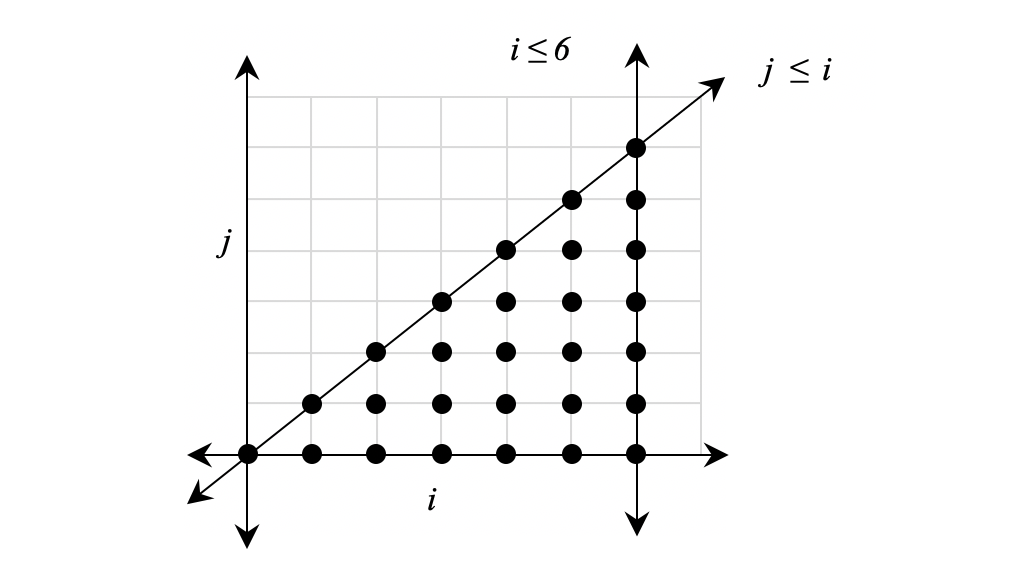
\includegraphics[scale=.48]{iteration_space.png}}
\end{adjustbox}
\caption{Polyhedral iteration space for prefix-sum}
\label{fig}
\end{figure}
The data space is usually one or more dimensions less than the iteration space. As a result, the data access functions are many-to-one mappings from iteration to data space. However, they are affine, leading to the model's clean closure properties under program transformation.

Going back to the original equation, a concise way to look at this computation would be to view it as an equation $\displaystyle sum[i] = \sum_{j=0}^{i}array[j]$.  The idea behind a polyhedral tool like \alphaz\ is exactly the reverse. It allows users to express one or more system of affine recurrence equations as a program, transform them using the polyhedral transformations that reduce the complexity of the program, use a better processor and memory allocation and then produce code for a language of interest.

\subsection{\uppercase{ALPHAZ}}
\alfa\ is a strongly typed functional language that works on a system of affine recurrence equations defined over polyhedral domains. Maurus~\cite{Mauras1989}  proposed this equational programming language as part of his doctoral dissertation.   Subsequently, it has been extended to include subsystems and reductions~\cite{leverge-thesis, leverge-parle92, fdupont-asap96, florent-thesis, DupontQuRi93}. Feautrier~\cite{feautrier91} showed that a polyhedral segment of code shown in Listing~\ref{listing:scan} can be translated to an \alfa\ program. \alfa\ is richer, mathematically cleaner, and more natural, especially, but not exclusively due to reductions.  \alphaz\ is the tool that allows program transformations and user-directed compilation of \alfa\ programs.  It provides a general framework for analysis, transformation, and code generation in polyhedral equational model.  \alphaz\ is similar to an earlier tool - \textsc{\texttt{MMAlpha}} , which targets field-programmable gate array based hardware design ~\cite{guillou-mma}. On the other hand, \alphaz\ targets code generation for multiprocessor shared-memory programs and focuses on programs with reduction operations. 

Every  \alfa\ program has two pieces – system definition and compilation script.  System definition of an  \alfa\ program allows users to express input and output of the program using polyhedral domains. 
It also allows a programmer to express the computation in terms of equations. The program containing the system definition is called alphabets. The second piece is the compilation script that contains commands to parse the input specification, transform the program based on the user input and finally generate the code. Algorithm~\ref{algo:matrix_mul_alphabets} highlights the alphabets program for matrix multiplication. Algorithm~\ref{algo:matrix_mul_script} presents a compiling script for matrix multiplication.
\begin{algorithm}
\caption{Matrix Multiplication in Alphabets}
\begin{algorithmic} [1]
\STATE \textbf{affine} MM $\lbrace N,K,M \mid (M, N, K)  > 0  \rbrace$
\STATE \textbf{input}
\STATE  \hspace{10pt} float A $\lbrace i, j \mid 0 \leq i < M \hspace{2pt} \&\& \hspace{2pt} 0 \leq j < K   \rbrace$ ;
\STATE  \hspace{10pt} float B $\lbrace i, j \mid 0 \leq i < K \hspace{2pt} \&\& \hspace{2pt} 0 \leq j < N   \rbrace$ ;
\STATE \textbf{output}
\STATE  \hspace{10pt} float C $\lbrace i, j \mid 0 \leq i < M \hspace{2pt} \&\& \hspace{2pt} 0 \leq j < N   \rbrace$;
\STATE \textbf{local}
\STATE \hspace{10pt} \slash \slash \text{local variables}
\STATE \textbf{output}
\STATE \hspace{10pt} C[$i,j$] = reduce(+, \hspace{2pt} [$k$], \hspace{2pt} A[$i,k$] * B[$k,j$]);
\end{algorithmic}
\label{algo:matrix_mul_alphabets}
\end{algorithm}
\subsubsection{Program Parsing}
The first step is to read the alphabets program, which decomposes the equations into abstract syntax tree notation internally and sets up the stage for various program transformations.
\subsubsection{Program Transformation}
All transformations in \alphaz\ are semantic preserving. However, it is the responsibility of the user to ensure the transformations are valid. \textit{Normalize} is the most basic transformation. It normalizes expression into normal form as per definition and makes the program easier to read and understand. \textit{NormalizeReduction} transforms unnormalized form to normalize form. A normal form of a reduction transforms the reduce-expression to be a direct child of an equation.  \textit{setSpaceTimeMap} allows the user to specify schedule and processor allocation to specify the order in which one or more processors visit the iteration space. A system with multiple variables requires the dimension of all the spacetime maps to be equal. \textit{NormalizeReduction} generates additional variables associated with the reductions. Specifying the schedule for such variable requires two different schedules to be provided – the first one specifies the order in which the iteration space will be visited.
 \begin{algorithm}
 \caption{Matrix Multiplication Command Script}
 \begin{algorithmic} [1]
 \STATE \text{\slash \slash \hspace{2pt}$Step-1: Parse \hspace{2pt} Alphabet \hspace{2pt} $}
 \STATE \text{prog=ReadAlphabets("MM.ab");}
 \STATE \text{system = “MM”;}
 \STATE \text{outDir="./src";}

 \STATE \text{}
 \STATE \text{\slash \slash \hspace{2pt}$Step-2: Perform \hspace{2pt} polyhedral \hspace{2pt}  transformation$}
 \STATE \text{Normalize(prog);}
 \STATE \text{setSpaceTimeMap(prog,  system,  “C”,  }
 \STATE \text{\hspace{140pt}"($i,j,k \mapsto i, k, j$)”,}
 \STATE \text{\hspace{140pt}“($i,j \mapsto i, -1, j$)”);}
 \STATE \text{setParallel(prog,  system,  “”,  "0" );}
 \STATE \text{}
 \STATE \text{\slash \slash \hspace{2pt}$Step-3: Generate  \hspace{2pt} code$}
 \STATE \text{generateWriteC(prog,  system,  outDir);}
\STATE \text{generateScheduleC(prog,  system,  outDir);}
\end{algorithmic}
\label{algo:matrix_mul_script}
\end{algorithm}
The other specifies the time at which the initialization should occur before starting the reduction. It also has a dependency on the schedule. \textit{setMemoryMap} - Memory map is a mapping between iteration points in the domain to the memory location. By default, \alphaz\ uses identity function as a memory map for each variable and bounding box of the polyhedral representation of the variable for storage. It allows multiple variables with different dimensions to share the same memory map based on affine function. \textit{setMemorySpace} is similar to memory map. Except that multiple variables with the same dimension can share memory space. \textit{setParallel} allows the user to specify one or more dimensions of the schedule to be executed in parallel by different threads. Users can also specify predicate as an ordering dimension to define the parallel loop dimension. Tiling transformation allows the user to chop the iteration space to improve data locality and adjust parallelization granularity.


\subsubsection{Code Generation}
This set of commands produce target code (e.g., c) based on the program transformation. \alphaz\ has various code generation options like – \textit{generateWriteC} which is sequential in nature and useful to check the correctness of the program, schedule code generation – \textit{generateScheduleC}. Sequential code generation hardly requires any
\begin{lstlisting}[language=Caml, caption=Generated code - Matrix multiplication]
    #define S1(i,j,i2) C(i,i2) = 0.0
    #define S0(i0,i1,i2) C(i0,i2) = (C(i0,i2))+((A(i0,i1))*(B(i1,i2)))
    {
        int c1,c2,c3;
        #pragma omp parallel for private(c2,c3)
        for(c1=0;c1 <= M-1;c1+=1){
	        for(c3=0;c3 <= N-1;c3+=1){
	            S1((c1),(-1),(c3));
	        }
            for(c2=0;c2 <= K-1;c2+=1){
                for(c3=0;c3 <= N-1;c3+=1){
                    S0((c1),(c2),(c3));
                }
            }
        }
    }
\end{lstlisting}
program transformation. However, efficient schedule code generation depends on the choice of various transformations, mainly the target mapping-related transformations. The tiling transformation is not applied upfront rather invoked as part of the post processing phase of the schedule code generation. 
%Please refer to Kim et al. \cite{Kim2010} for more details on tiling code generation algorithm.

%\Comment{Haven't read beyond this}
\section{METHODS} \label{section:methods}
We have staged our optimization process into three distinct phases.  The following subsections describe these phases.

\subsection{Phase-1:}
This phase's primary goal is to express the BPMax equation in \alphaz\ , perform the first-level optimization on the most compute-intensive portion of the task and get a baseline estimation.

\paragraph{Multi-dimensional Affine Schedule for Double Max-plus Operation}
We simplify the BPMax computation based on the following recurrence equation as the very first step.
\begin{equation}
\label{eqn:double_max_plus_recurrence}
F_{i_{1},j_{1},i_{2},j_{2}} \\ = 
                 {\max\limits_{k_{1}=i_{1}}^{j_{1}-1} \max\limits_{k_{2}=i_{2}}^{j_{2}-1} F_{i_{1},k_{1}, i_{2}, k_{2}}+ F_{k_{1}+1,j_{1}, k_{2}+1, j_{2}}}\\
            \\
\end{equation}
Let us call this double max-plus computation $R_{0}$. Our goal is to find out the optimum multi-dimensional affine schedule \cite{feautrier92a, feautrier92b}  for this equation. A schedule is only valid if it preserves the program semantic, which requires dependency analysis. We observe that each inner triangle of $F$-table is dependent on the triangles to the west and south. E.g., triangle $C$ is dependent on all the $Ax$ triangles towards the west and $Bx$ triangles towards the south illustrated in Figure~\ref{fig:double_plus_dependencies}. There is no dependency from the triangle within. So, each inner triangle can be filled diagonally or bottom-up and then left to right. The first two dimensions of our multi-dimensional schedule can be either $(j_{1}-i_{1}, i_{1})$ or $(M-i_{1}, j_{1})$ or $(-i_{1}, j_{1})$ for $F$-table and $R_{0}$. There are many ways to formulate the next dimension for $R_{0}$. One such choice would be to use $k_{1}$. Figure~\ref{fig:double_max_plus_accumulation_sequence} highlights the accumulation sequence based on this choice. It has the effect of performing multiple max-plus operations on a series of matrices $( i_{1}, k_{1})$ and $(k_{1}+1, j_{1})$. It requires the third dimension of the $F$-table to be $j_{1}$, meaning we must finish computing all the max-plus operations for the current triangle before updating it. The inner three dimensions of the $R_{0}$ can be in any order since they do not have any dependencies.
\begin{figure}[htbp]
\begin{adjustbox}{varwidth=\textwidth,margin=0 {\abovecaptionskip} 0 0, frame=0.00pt}
\centerline{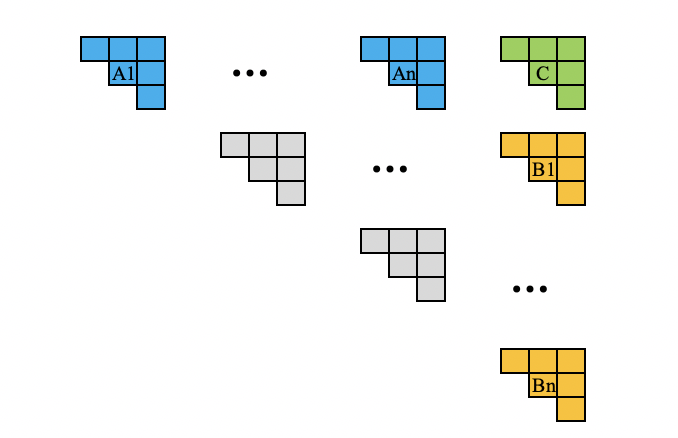
\includegraphics[scale=.74]{double_max_plus_dependence.png}}
\end{adjustbox}
\caption{Double max-plus dependency}
\label{fig:double_plus_dependencies}
\end{figure}
Thus, it can be $(j_{2}-i_{2}, i_{2}, k_{2})$ or $(i_{2}, j_{2}, k_{2})$ or $(M-i_{2}, j_{2}, k_{2})$ or $(i_{2}, j_{2}, k_{2})$ or $(j_{2}-i_{2}, k_{2}, i_{2})$ or $(-i_{2}$, $k_{2}$, $j_{2}$) etc.  However, auto-vectorization is prohibited if $k_{2}$ is the innermost loop iteration. 
\begin{figure}[htbp]
\begin{adjustbox}{varwidth=\textwidth,margin=0 {\abovecaptionskip} 0 0, frame=0.00pt}
\centerline{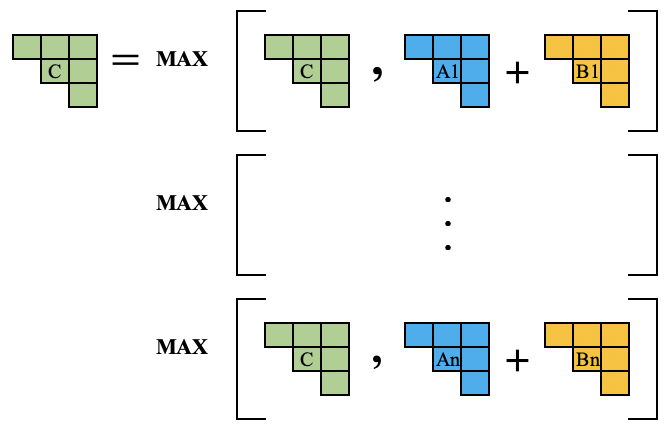
\includegraphics[scale=.74]{double_max_plus_accumulation_sequence.png}}
\end{adjustbox}
\caption{Double max-plus accumulation sequence}
\label{fig:double_max_plus_accumulation_sequence}
\end{figure}
Other choices can be viewed as loop permutations that allow auto-vectorization. For updating the final $F$-table entries, we can copy the data in any order. The original BPMax implementation uses $ i_{1},j_{1},i_{2},j_{2} \mapsto j_{1}-i_{1},j_{2}-i_{2},i_{1}, i_{2},k_{1},k_{2} $ schedule for double max-plus computation. 
Table~\ref{tab1:double_max_plus_schedule}  
shows various multi-dimensional affine schedules similar to Varadrajan’s. We pick similar schedules to establish the baseline since her kernel was based on multiply-add and ours is max-plus. Also, we use single-precision storage to reduce the memory footprint of BPMax.

\paragraph{Machine Peak Analysis and Micro-benchmark}
Next, we develop the roofline model for the target machine. Our schedule tries to exploit auto-vectorization that loads one scalar and vector of $8$ elements from L1 to compute $8$ max-plus operations, and the data access pattern is $ Y = \max (a+X, Y)$. We create a micro-benchmark to estimate the attainable L1 bandwidth for such access pattern. It allocates two large one-dimensional arrays for each thread, initializes them with random numbers, and
\begin{algorithm}
\caption{Max-plus streaming benchmark}
\label{algo:sequential_bench_mark}
\begin{algorithmic} [1]
  \FOR{$iteration \gets 0, MAX\_ITERATION$}
     \FOR{$index \gets 0, CHUNK\_SIZE$} 
     \STATE{$Y[index] = \max(alpha+X[index], Y[index])$} 
     \ENDFOR
  \ENDFOR 
\end{algorithmic}
\end{algorithm}
 then invokes the kernel (Algorithm~\ref{algo:sequential_bench_mark}) that computes the max-plus operation on the array.  The micro-benchmark data is presented in the result section.


\begin{table}[htbp]
\caption{\uppercase{Double max-plus schedule}}
\begin{center}
\begin{tabular}{|c|c|c|}
\hline
\textbf{} & \textbf{\textit{Variable}}& \textbf{\textit{Schedule}} \\
\hline
  & $F$ & $(i_{1},j_{1},i_{2},j_{2} \mapsto j_{1}-i_{1},i_{1},j_{1},i_{2},j_{2},j_{2})$   \\
\cline{2-3} 
$^{\mathrm{a}}$ & $R_{0}$ & $(i_{1},j_{1},i_{2},j_{2},k_{1},k_{2} \mapsto j_{1}-i_{1},i_{1},k_{1},i_{2},k_{2},j_{2})$,    \\
 & & $(i_{1},j_{1},i_{2},j_{2} \mapsto j_{1}-i_{1},i_{1},i_{1}-1,i_{2},i_{2}-1,j_{2})$ \\
\hline
  & $F$ & $(i_{1}, j_{1}, i_{2}, j_{2} \mapsto -i_{1}, j_{1}, j_{1}, -i_{2}, j_{2}, j_{2})$  \\
\cline{2-3} 
$^{\mathrm{b}}$ & $R_{0}$& $(i_{1},j_{1},i_{2},j_{2},k_{1},k_{2} \mapsto -i_{1},j_{1},k_{1},-i_{2},k_{2},j_{2})$ ,   \\
 & & $(i_{1},j_{1},i_{2},j_{2} \mapsto -i_{1},j_{1},i_{1}-1,-i_{2},i_{2}-1,j_{2})$ \\
\hline
  & $F$ & $(i_{1}, j_{1}, i_{2}, j_{2} \mapsto  j_{1}-i_{1}, i_{1}, j_{1}, i_{2}, j_{2}, j_{2})$   \\
\cline{2-3} 
$^{\mathrm{c}}$ & $R_{0}$& $(i_{1},j_{1},i_{2},j_{2},k_{1},k_{2} \mapsto j_{1}-i_{1},i_{1},k_{1},i_{2},k_{2},j_{2})$ ,   \\
 & & $(i_{1},j_{1},i_{2},j_{2} \mapsto j_{1}-i_{1},i_{1},i_{1}-1,i_{2},i_{2}-1,j_{2})$ \\
\hline
\multicolumn{3}{l}{$^{\mathrm{a}}$Fine-grain schedule(diagonal), parallel dimension 3}\\
\multicolumn{3}{l}{$^{\mathrm{b}}$Fine-grain schedule(bottom-up), parallel dimension 3}\\
\multicolumn{3}{l}{$^{\mathrm{c}}$Coarse-grain schedule, parallel dimension 1}
\end{tabular}
\label{tab1:double_max_plus_schedule}
\end{center}
\end{table}


\paragraph{Insights from Phase-I}
This phase highlights the possibility of further improvements of $R_{0}$ beyond loop permutation. Double max-plus performance attains just above  $20\%$ of our theoretical max-plus machine peak. We notice a significant collapse in performance when the input sequences are longer.
 
\subsection{Phase-II}
We have two objectives in this phase. First, find a complete schedule for BPMax that enables automatic vectorization for all the variables and estimate the other reduction term's overhead. Second, explore optimization opportunities for the double max-plus operation.
 
\paragraph{Multi-Dimensional Affine Schedule for BPMax}
Figure~\ref{fig:bpmax_dependency} shows the complete BPMax dependencies for a point. The point colored in red depends on all the other colored points.  BPMax has a total of five reductions. There are four additional reductions $R_{1}$ (green), $R_{2}$ (orange), $R_{3}$ (purple), $R_{4}$ (yellow) beside $R_{0}$ (blue). So, there are new dependencies in addition to the similar dependencies highlighted in the double max-plus computation. $R_{1}$ and $R_{2}$  have internal dependencies, but the other two have external dependencies. One common theme across various schedules is that $S^{(1)}$ and $S^{(2)}$ can be scheduled before scheduling any other variables. Also, order of filling up the inner triangle does not change with the introduction of the other terms. Thus, the first two dimensions of our multi-dimensional schedule can be either $(j_{1}-i_{1}, i_{1})$ or $(M-i_{1}, j_{1})$ or $(-i_{1}, j_{1})$ for $F$-table, $R_{0}$, $R_{1}$, $R_{2}$, $R_{3}$, $R_{4}$. $R_{3}$ and $R_{4}$ is over $k_{1}$ like $R_{0}$. So, the third dimension can be the same for all of them. Next, the inner three dimensions of the $R_{0}$ can also be the same as discussed earlier. $R_{3}$ and $R_{4}$  can use $(i_{2}, j_{2})$. However, we introduce additional terms to make the schedule dimension equal for all the variables. $F$-table, $R_{1}$, and $R_{2}$ must wait until $k_{1}$ reaches $j_{1}$ like double max-plus. 
\begin{figure}[htbp]
\begin{adjustbox}{varwidth=\textwidth,margin=0 {\abovecaptionskip} 0 0, frame=0.00pt}
\centerline{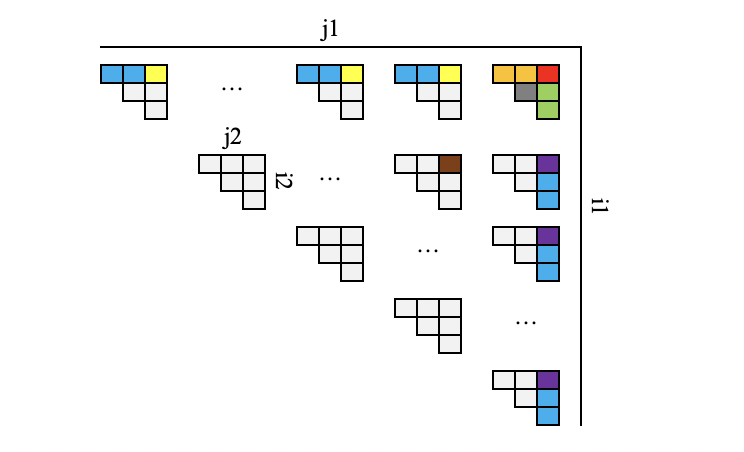
\includegraphics[scale=.66]{bpmax_dependency_new.png}}
\end{adjustbox}
\caption{BPMax dependency overview}
\label{fig:bpmax_dependency}
\end{figure}
 Thus, their third schedule dimension becomes $j_{1}$. Final $F$-table entries require intra-triangular dependencies to be evaluated which are similar to inter-triangular dependencies. So, it can be filled up diagonally or bottom-up and left to right.
\begin{table}[htbp]
\caption{\uppercase{BPMax fine-grain schedule}}
\begin{center}
\begin{tabular}{|c|c|}
\hline
\textbf{\textit{Variable}}& \textbf{\textit{Schedule}}$^{\mathrm{a}}$ \\
\hline
  $S^{(1)}, S^{(2)}$ & $(i_{1},j_{1} \mapsto 0, 0, 0, 0, j_{1}-i_{1}, i_{1}, 0, 0)$   \\
\cline{1-2} 
  $F$ & $(i_{1},j_{1},i_{2},j_{2} \mapsto 1, -i_{1}, j_{1}, j_{1}, -i_{2}, 0, j_{2},0)$   \\
\cline{1-2} 
$R_{1}, R_{2}$ & $(i_{1},j_{1},i_{2},j_{2},k_{2} \mapsto 1, -i_{1}, j_{1}, j_{1}, -i_{2}, 0, k_{2}, j_{2})$,    \\
 & $(i_{1},j_{1},i_{2},j_{2} \mapsto 1, -i_{1}, j_{1}, j_{1}, -i_{2}, 0, i_{2}-1, j_{2})$ \\
 \cline{1-2} 
 $R_{0}$ & $(i_{1},j_{1},i_{2},j_{2},k_{1},k_{2} \mapsto 1, -i_{1}, j_{1}, k_{1}, -1, -i_{2}, k_{2}, j_{2})$,    \\
  & $(i_{1},j_{1},i_{2},j_{2} \mapsto 1, -i_{1}, j_{1}, i_{1}-1, -1, -i_{2}, i_{2}-1, j_{2})$ \\
\cline{1-2} 
 $R_{3}, R_{4}$ & $(i_{1},j_{1},i_{2},j_{2},k_{1} \mapsto 1, -i_{1}, j_{1}, k_{1}, -1, -i_{2}, i2, j_{2})$,    \\
 & $(i_{1},j_{1},i_{2},j_{2} \mapsto 1, -i_{1}, j_{1}, i_{1}-1, -1, -i_{2}, i_{2}, j_{2})$ \\
 \cline{1-2} 
\hline
\multicolumn{2}{l}{$^{\mathrm{a}}$Parallel dimension 5}
\end{tabular}
\label{tab:bpm_fine_grain_schedule}
\end{center}
\end{table}
\begin{table}[htbp]
\caption{\uppercase{BPMax coarse-grain schedule}}
\begin{center}
\begin{tabular}{|c|c|}
\hline
\textbf{\textit{Variable}}& \textbf{\textit{Schedule}}$^{\mathrm{a}}$ \\
\hline
  $S^{(1)}, S^{(2)}$ & $(i_{1},j_{1} \mapsto 0, j_{1}-i_{1}, i_{1}, 0, 0, 0, 0)$   \\
\cline{1-2} 
  $F$ & $(i_{1},j_{1},i_{2},j_{2} \mapsto 1, j_{1}-i_{1}, i_{1}, j_{1}, -i_{2}, j_{2}, j_{2}$   \\
\cline{1-2} 
$R_{1}, R_{2}$ & $(i_{1},j_{1},i_{2},j_{2},k_{2} \mapsto 1, j_{1}-i_{1}, i_{1}, j_{1}, -i_{2}, k_{2}, j_{2})$ ,   \\
 & $(i_{1},j_{1},i_{2},j_{2} \mapsto 1, j_{1}-i_{1}, i_{1}, j1, -i_{2}, i_{2}-1, j_{2})$ \\
 \cline{1-2} 
$R_{0}$ & $(i_{1},j_{1},i_{2},j_{2},k_{1},k_{2} \mapsto 1, j_{1}-i_{1}, i_{1}, k_{1}, i_{2}, k_{2}, j_{2})$,    \\
 & $(i_{1},j_{1},i_{2},j_{2} \mapsto 1, j_{1}-i_{1}, i_{1}, i_{1}-1, i_{2}, i_{2}-1, j_{2})$ \\
\cline{1-2} 
$R_{3}, R_{4}$ & $(i_{1},j_{1},i_{2},j_{2},k_{1} \mapsto 1, j_{1}-i_{1}, i_{1}, k_{1}, i_{2}, i_{2}, j_{2})$,    \\
 & $(i_{1},j_{1},i_{2},j_{2} \mapsto 1, j_{1} -i_{1}, i_{1}, i_{1}-1, i_{2}, i_{2}, j_{2})$ \\
 \cline{1-2} 
\hline
\multicolumn{2}{l}{$^{\mathrm{a}}$Parallel Dimension 2}
\end{tabular}
\label{tab:bpm_coarse_grain_schedule}
\end{center}
\end{table}
Thus, the inner three dimensions of the schedule for $R_{1}$ and $R_{2}$ can be $(j_{2}-i_{2}, i_{2}, k_{2})$ or $(N-i_{2}, j_{2}, k_{2})$ or $(-i_{2}, j_{2}, k_{2})$ or $(j_{2}-i_{2}, k_{2}, j_{2})$ or $(N-i_{2}, k_{2}, j_{2})$ or $(-i_{2}, k_{2}, j_{2})$ etc. We carefully chose the schedule for $R_{1}$ and $R_{2}$ since the innermost $k_{2}$ prevents automatic vectorization.  We  ensure that $F$-table gets updated when $k_{2}$ reaches $j_{2}$. Table~\ref{tab:bpm_fine_grain_schedule} and ~\ref{tab:bpm_coarse_grain_schedule}  shows various multi-dimensional affine schedules which provide better results than the base schedule.  
 
\paragraph{Parallelization Approach} 
We take two different types of parallelization approach in this phase - coarse and fine-grain. For coarse-grain parallelization, threads work on distinct inner triangles simultaneously.  It is valid for $R_{0}$, $R_{1}$, $R_{2}$, $R_{3}$, and $R_{4}$. On the other hand, threads work on individual rows of an inner triangle simultaneously for fine-grain parallelization. It is only valid for $R_{0}$, $R_{3}$, and $R_{4}$. 



\paragraph{Memory Optimization} 
Memory-overhead of our \alphaz\ generated code is $M^2 \times N^2$. However, we only need one-fourth of that memory. Even though it seems inefficient, the unused elements are never moved between memory hierarchies. Reduction variables also take up memory space by default, which is wasteful. In this phase, coarse-grain parallelization still requires $P$ (number of threads) instances of a $2-D$ array for each reduction variables to be active in memory except $R_{0}$.
\begin{figure}[htbp]
\begin{adjustbox}{varwidth=\textwidth,margin=0 {\abovecaptionskip} 0 0, frame=0.00pt}
\centerline{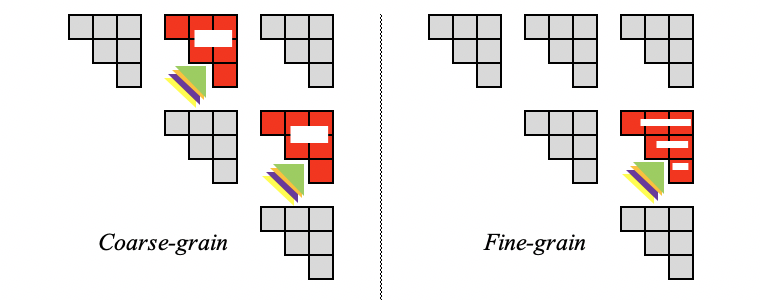
\includegraphics[scale=.585]{bpm_phase_2_memory_map.png}}
\end{adjustbox}
\caption{BPMax phase-II memory map}
\label{fig:bpm_phase_2_memory_map}
\end{figure}
$R_{0}$ shares memory with $F$. Fine-grain requires only a $2-D$ array for each of these variables illustrated in Figure~\ref{fig:bpm_phase_2_memory_map}.
 
\paragraph{Tiling $R_{0}$} 
The fine-grain parallelism for the $R_{0}$ assigns one or more rows to each thread. Processing each row needs to access one complete inner triangle below that row before moving to the next.  
\begin{figure}[htbp]
\begin{adjustbox}{varwidth=\textwidth,margin=0 {\abovecaptionskip} 0 0, frame=0.00pt}
\centerline{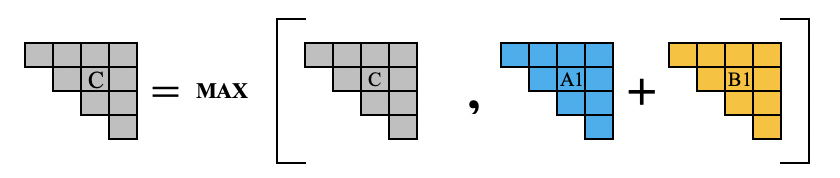
\includegraphics[scale=.57]{single_max_plus_operation.png}}
\end{adjustbox}
\caption{A matrix instance of max-plus operation}
\label{fig:matrix_instance_max_plus}
\end{figure}
It motivates us to tile computations of one matrix instance of max-plus operation. It is matrix multiplication like computation, except only a fraction of work is being done here, and the access pattern is imbalanced. We tile three inner dimensions with $k_{2}$ loop still in the middle and $j_{2}$ loop inside. So, this chops $(i_{2}, k_{2}, j_{2})$ iteration space, and we parallelize the outer $i_{2}$ dimension.

 \paragraph{Insights from Phase-II} 
Loop permutation and automatic vectorization provide a significant speedup for the entire BPMax program. However, the program suffers from imbalanced parallelization. The tiled version of the $R_{0}$ attains $33\%$ of our theoretical max-plus machine peak.

\subsection{Phase-III}
In this phase, we handle the load imbalance between threads and partially ($R_{0}$, $R_{3}$, $R_{4}$) apply tiling to BPMax.

\paragraph{Parallelization Approach}
Earlier, we have observed that the program quickly becomes DRAM-bound for the coarse-grain schedule since each thread computes an inner triangle. But, it allows us to parallelize $R_{1}$ and $R_{2}$.  On the other hand, $R_{0}$, $R_{3}$, and $R_{4}$ can be computed using the fine-grain schedule, which reduces data movement between DRAM and LLCs. However, $R_{1}$ and $R_{2}$ are not easy to parallelize.
\begin{table}[htbp]
\caption{\uppercase{BPMax hybrid schedule}}
\begin{center}
\begin{tabular}{|c|c|}
\hline
\textbf{\textit{Variable}}& \textbf{\textit{Schedule}}$^{\mathrm{a}}$ \\
\hline
 $S^{(1)}, S^{(2)}$ & $(i_{1},j_{1} \mapsto 0, 0, 0, j_{1}-i_{1}, i_{1}, 0, 0, 0)$   \\
\cline{1-2} 
 $F$ & $(i_{1},j_{1},i_{2},j_{2} \mapsto 1, j_{1}-i_{1}, M, 0, i_{1}, -i_{2}, j_{2}, 0$   \\
\cline{1-2} 
$R_{1}, R_{2}$ & $(i_{1},j_{1},i_{2},j_{2},k_{2} \mapsto 1, j_{1}-i_{1}, M, 0, i_{1}, -i_{2}, k_{2}, j_{2})$ ,   \\
 & $(i_{1},j_{1},i_{2},j_{2} \mapsto 1, j_{1}-i_{1}, M, 0, i_{1}, -i_{2}, i_{2}-1, j_{2})$ \\
 \cline{1-2} 
$R_{0}$ & $(i_{1},j_{1},i_{2},j_{2},k_{1},k_{2} \mapsto 1, j_{1}-i_{1}, i_{1}, k_{1}, i_{2}, k_{2}, j_{2}, 0)$,    \\
 & $(i_{1},j_{1},i_{2},j_{2} \mapsto 0, j_{1}-i_{1}, i_{1}, 0, i_{2}, 0, j_{2}, 0)$ \\
\cline{1-2} 
$R_{3}, R_{4}$ & $(i_{1},j_{1},i_{2},j_{2},k_{1} \mapsto 1, j_{1}-i_{1}, i_{1}, k_{1}, i_{2}, i_{2}, j_{2},0)$,    \\
 & $(i_{1},j_{1},i_{2},j_{2} \mapsto 0, j_{1}-i_{1}, i_{1}, 0, i_{2}, 0, j_{2}, 0)$ \\
 \cline{1-2} 
\hline
\multicolumn{2}{l}{$^{\mathrm{a}}$Parallel Dimension 4}
\end{tabular}
\label{tab:hybrid_schedule}
\end{center}
\end{table}
These are optimum string parenthesization (OSP)-like computations that require further transformation like middle serialization. If we use the fine-grain parallelism without such transformation, only one thread stays active, leading to lower CPU resource utilization. We take advantage of the best of both worlds. We use the fine-grain parallelism for $R_{0}$, $R_{3}$, $R_{4}$ and the coarse-grain parallelism for $F$-table, $R_{1}$, $R_{2}$. We call this hybrid schedule shown in Table ~\ref{tab:hybrid_schedule}. It improves CPU utilization and limits the data movement between DRAM and LLCs. However, there are some limitations discussed in the result section.


\paragraph{Tiling Integration and Subsystem Scheduling}
\alphaz\ produces inferior code when the tiling is applied to a subset of reduction operations. 
\begin{table}[htbp]
\caption{\uppercase{BPMax hybrid schedule with tiling}}
\begin{center}
\begin{tabular}{|c|c|c|}
\hline
\textbf{} & \textbf{\textit{Variable}}& \textbf{\textit{Schedule}} \\
\hline
 & ${\mathrm{c}}$& $(i_{1},j_{1} \mapsto M, i_{1}, j_{1}, 0)$ \\
 \cline{2-3} 
${\mathrm{a}}$ & $R_{0}$ & $(i_{1},j_{1},k_{1},k_{2} \mapsto k_{1}, i_{1}, k_{2}, j_{1})$,    \\
 & & $(i_{1},j_{1} \mapsto -1, i_{1}, 0, j_{1})$ \\
\cline{2-3} 
& $R_{3}, R_{4}$ & $(i_{1},j_{1},k_{1} \mapsto k_{1}, i_{1}, i_{1}, j_{1})$,    \\
 & & $(i_{1},j_{1} \mapsto -1, i_{1}, 0, j_{1})$ \\
 \cline{2-3} 
\hline
& $S^{(1)}, S^{(2)}$ & $(i_{1},j_{1} \mapsto 0, 0, j_{1}-i_{1}, i_{1}, 0, 0, 0)$   \\
\cline{2-3} 
& ${\mathrm{d}}$ & $(i_{1},j_{1} \mapsto 1, j_{1}-i_{1}, i_{1}, j_{1}-4, 0, 0, 0)$   \\
\cline{2-3} 
${\mathrm{b}}$ & $F$ & $(i_{1},j_{1},i_{2},j_{2} \mapsto 1, j_{1}-i_{1}, M, i_{1}, -i_{2}, j_{2}, 0)$   \\
\cline{2-3} 
& $R_{1}, R_{2}$ & $(i_{1},j_{1},i_{2},j_{2},k_{2} \mapsto 1, j_{1}-i_{1}, M, i_{1}, -i_{2}, k_{2}, j_{2})$ ,   \\
 & & $(i_{1},j_{1},i_{2},j_{2} \mapsto 1, j_{1}-i_{1}, M, i_{1}, -i_{2}, i_{2}-1, j_{2})$ \\
\hline
\multicolumn{3}{l}{}\\
\multicolumn{3}{l}{${\mathrm{a}}$ - Subsystem schedule(parallel dimension 1)}\\
\multicolumn{3}{l}{${\mathrm{b}}$ - Root system schedule(parallel dimension 3)}\\
\multicolumn{3}{l}{${\mathrm{c}}$ - Subsystem output}\\
\multicolumn{3}{l}{${\mathrm{d}}$ - Subsystem call}\\
\end{tabular}
\label{tab:hybrid_schedule_with_tiling}
\end{center}
\end{table}
It is due to the insertion of additional schedule dimensions needed to isolate the tiling band. So, we use \alfa\ subsystem, which partitions BPMax computation into two systems. The subsystem produces an inner triangle using $R_{0}$, $R_{3}$, $R_{4}$ and the primary system produces $R_{1}$ and $R_{2}$ along with final $F$-table output and consolidates the results from the subsystem. It allows us to modularize the program and apply tiling transformation on $R_{0}$, $R_{3}$, and $R_{4}$ efficiently. The subsystem gets called for each instance of an inner $F$-table update.  Finally, \textit{use equation} construct integrates these two systems. We invoke the subsystem call for each instance of the iteration space defined by the schedule's first two dimensions. Now, this requires us to specify the schedule for the subsystem invocation. Both systems are integrated manually. We perform minimal preprocessing since our code generator can not produce tiled code for the subsystem automatically. Two lines of source code changes are made to achieve this. Table~\ref{tab:hybrid_schedule_with_tiling} summarizes the complete schedule for the two systems.

 
\paragraph{Memory Optimization}
We further optimize memory utilization in this phase. $R_{0}$, $R_{3}$ and $R_{4}$ are always computed before final $F$-table update. So, they share the memory with $F$-table. 
\begin{figure}[htbp]
\begin{adjustbox}{varwidth=\textwidth,margin=0 {\abovecaptionskip} 0 0, frame=0.00pt}
\centerline{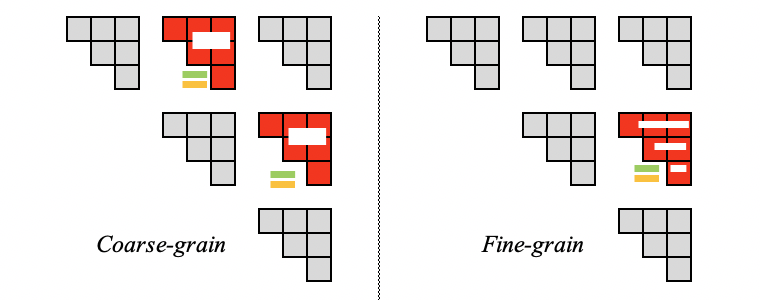
\includegraphics[scale=.63]{bpm_phase_3_memory_map.png}}
\end{adjustbox}
\caption{BPMax phase-III memory map}
\label{fig:bpm_phase_3_memory_map}
\end{figure}
Also, only one row of an inner triangle is required for $R_{1}$ and $R_{2}$ to keep up with the $F$-table update. This has been highlighted in Figure ~\ref{fig:bpm_phase_3_memory_map}. We also optimize redundant data copies during subsystem call using \textit{setMemorySpaceForUseEquationOptimization} transformation. 

\paragraph{Performance Tuning}
To find an optimum tile shape, we start with cubic tiles and then adjust one or more dimensions to find a better tile shape that works moderately well across various inputs. However,  we notice 10\% performance differences between the best and generic tile sizes. 
\begin{figure}[htbp]
\begin{adjustbox}{varwidth=\textwidth,margin=0 {\abovecaptionskip} 0 0, frame=0.00pt}
\centerline{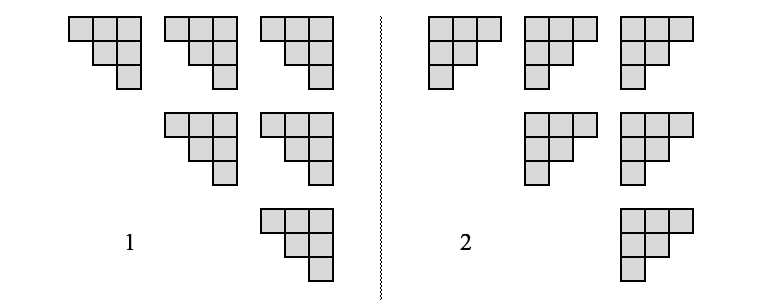
\includegraphics[scale=.63]{memory_map_update.png}}
\end{adjustbox}
\caption{Memory mapping schemes}
\label{fig:memory_map_schemes}
\end{figure}
The OMP dynamic-schedule works better than the static and guided-schedule due to an imbalanced workload. Next, we perform some manual memory optimization. The schedule initializes memory for each reduction body. Still, when one variable shares memory space with multiple variables,  memory initialization becomes redundant, and the current code generator does not optimize it. We comment out these macros, which attempt duplicate initializations to eliminate redundancies. We have tried two different memory transformations for the inner triangle highlighted in  Figure~\ref{fig:memory_map_schemes} - 1 : $(i_{2}, j_{2} \mapsto i_{2}, j_{2})$   and 2 : $(i_{2}, j_{2} \mapsto i_{2}, j_{2}-i_{2})$. Option-1 always performs better.

%\paragraph{Validation of Program Correctness}
%In addition to checking the final scores between reference and optimized version, 
%We use \alphaz\ toolset to verify the correctness of the optimized program using a verifier that compares outputs of a schedule code with sequential code. However, this is not sufficient due to max-plus operation.  We develop a parallel version of the BPMax program to replace the max-plus operation with plus-plus operation and apply the exact same sequence of transformations and ran it through the verifier to ensure that our transformations and schedules do not change the semantics of the original program. %One of the major challenge was to run the validation on longer sequences since the base and sequential implementations are extremely slow. 

%\paragraph{Validation of Program Correctness}
%In addition to checking the final scores between reference and optimized version, We use \alphaz\ toolset to verify the correctness of the optimized program using a verifier that compares outputs of a schedule code with the sequential code. %However, this is not sufficient due to max-plus operation.  We develop a parallel version of the BPMax program to replace the max-plus operation with plus-plus operation and apply the exact same sequence of transformations and ran it through the verifier to ensure that our transformations and schedules do not change the semantics of the original program. %One of the major challenge was to run the validation on longer sequences since the base and sequential implementations are extremely slow.

\section{RESULTS} \label{section:results}
We use Xeon E5-1650v4 to present the results of our optimization approach. Xeon E5-1650v4 has six cores where each core has 32 KB 8-way set associative L1 and 256 KB 8 way-set associative cache. They share a 15 MB 20-way set-associative cache.
\subsection{Machine Peak Overview}
Intel's micro-architecture specification indicates that the sustained L1 and L2 data cache bandwidth are $93$ bytes and $25$ bytes/cycle, respectively, whereas L3 bandwidth and DRAM
\begin{figure}[htbp]
\centerline{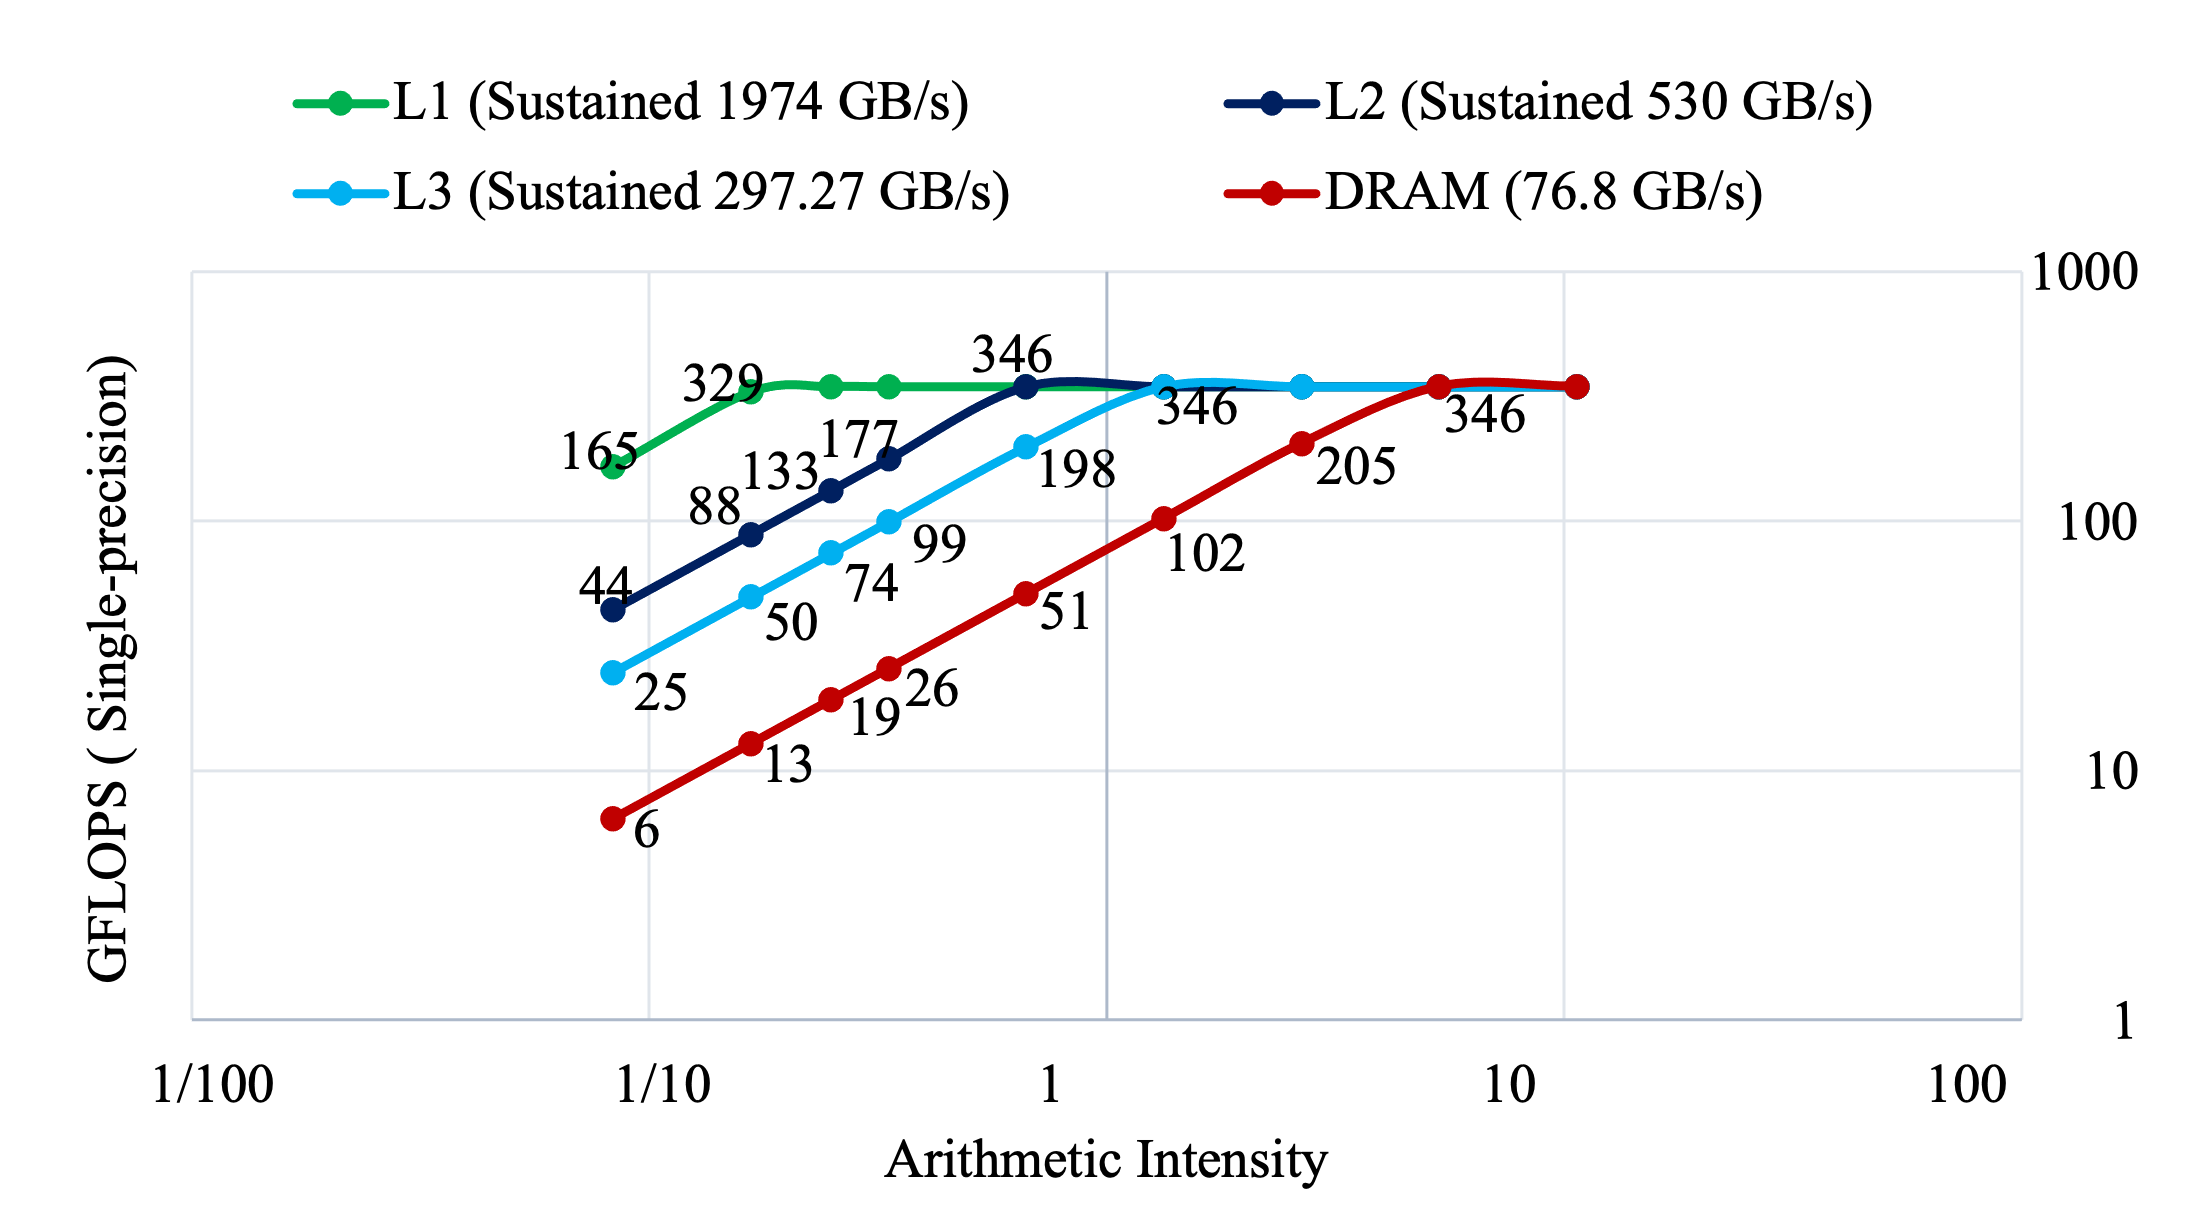
\includegraphics[scale=0.52, trim=5 5 5 5,clip]{figure_machine_roofline.png}}
\caption{Xeon E5 1650v4 roofline based on micro-architecture  }
%\caption{Xeon E5 1650v4 roofline based on micro-architecture  }
\label{fig:roof_line}
\end{figure}
bandwidth are $14$ bytes/cycle and $76.8$ GB/second,  respectively. Based on this data, we have come up with the roofline model shown in Figure~\ref{fig:roof_line}. The theoretical max-plus machine peak is about $346$ GFLOPS for single-precision. We will implicitly use GFLOPS to indicate the single-precision performance for the rest of the section. 
\begin{figure}[htbp]
\centerline{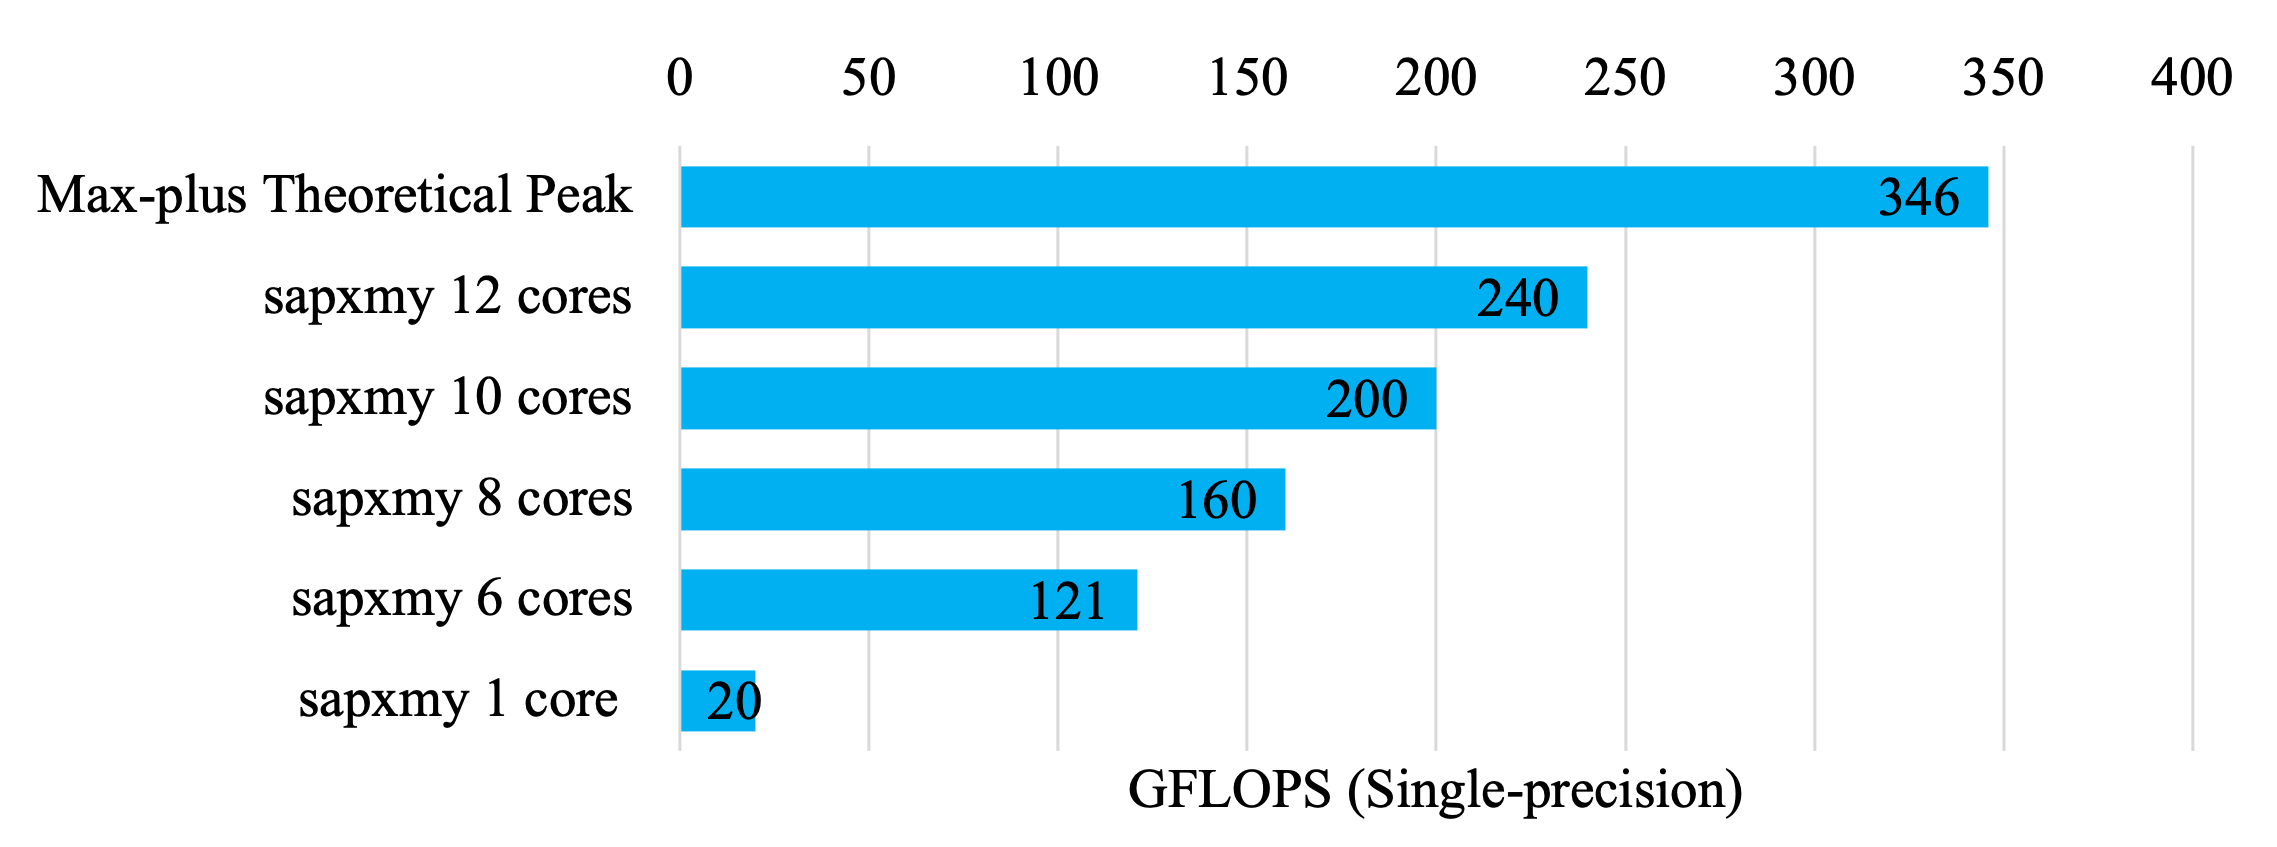
\includegraphics[scale=0.50, trim=5 5 5 5,clip]{figure_micro_benchmark.png}}
%\end{adjustbox}
\caption{Micro-benchmark for $Y= \max(a+X, Y)$}
\label{fig:micro_bench_mark}
\end{figure}
BPMax performs 2-arithmetic operations for 3-single-precision memory operations. So, its arithmetic intensity is $\frac{2}{(3 \times 4)}$ or $ \frac{1}{6}$ (second data points on each series shown in Figure~\ref{fig:roof_line}). Based on the roofline model, we expect to achieve around $329$ GFLOPS based on L1 bandwidth. Our micro-benchmark data (Figure~\ref{fig:micro_bench_mark}) shows that we achieve up to $120$ GFLOPS with $6$ threads and $240$ GFLOPS with $12$ threads.

\subsection{Performance Analysis of Double Max-plus Computation}
In this section, we go over the results of our optimization approach for double max-plus computation. Figure~\ref{fig:peroformance_analysis_double_max_plus} and  Figure~\ref{fig:double_max_plus_speed_up} show the performance and speedup comparison of double max-plus between different schedules using $6$ threads.  We see that the coarse-grain parallelization performs very poorly since it generates a lot of DRAM traffic and makes the program slower. There is a minor difference between computing the inner triangles of $F$-table diagonally vs. bottom-up and left to right highlighted in orange and blue. In both cases, all the threads work on one inner triangle before moving to the next. Our tiling approach improves locality and maintains automatic vectorization. It enables us to get close to the $97\%$ of our micro-benchmark target. We attain $117$ GFLOPS with the tiling transformation. Tile dimensions of $(32 \times 4 \times N)$ and $(64 \times 16 \times N)$ are used for presenting the performance and speedup comparison. $(32 \times 4 \times N)$ is restricted for sequence length up to 2048. 

We achieve around $178\times$ improvement over the base implementation taken from the BPMax program. It is a sequential improvement of $40-200\%$ with $6$ threads over Varadrajan’s fine-grain schedule. However, her results show that hyperthreading helped improve performance by over $10\%$ in some cases. We see minimal ($3-5\%$) improvement with hyper-threading over six threads shown in Figure~\ref{fig:hyperthreading_effect}. We have done experiments with different tile sizes ($ i_{2} \times k_{2} \times j_{2}$) and found that the cubic tiles perform poorly. We observe the best result when  $j_{2}$ is not tiled due to the streaming effect. 
\begin{figure*}[htbp]
\centerline{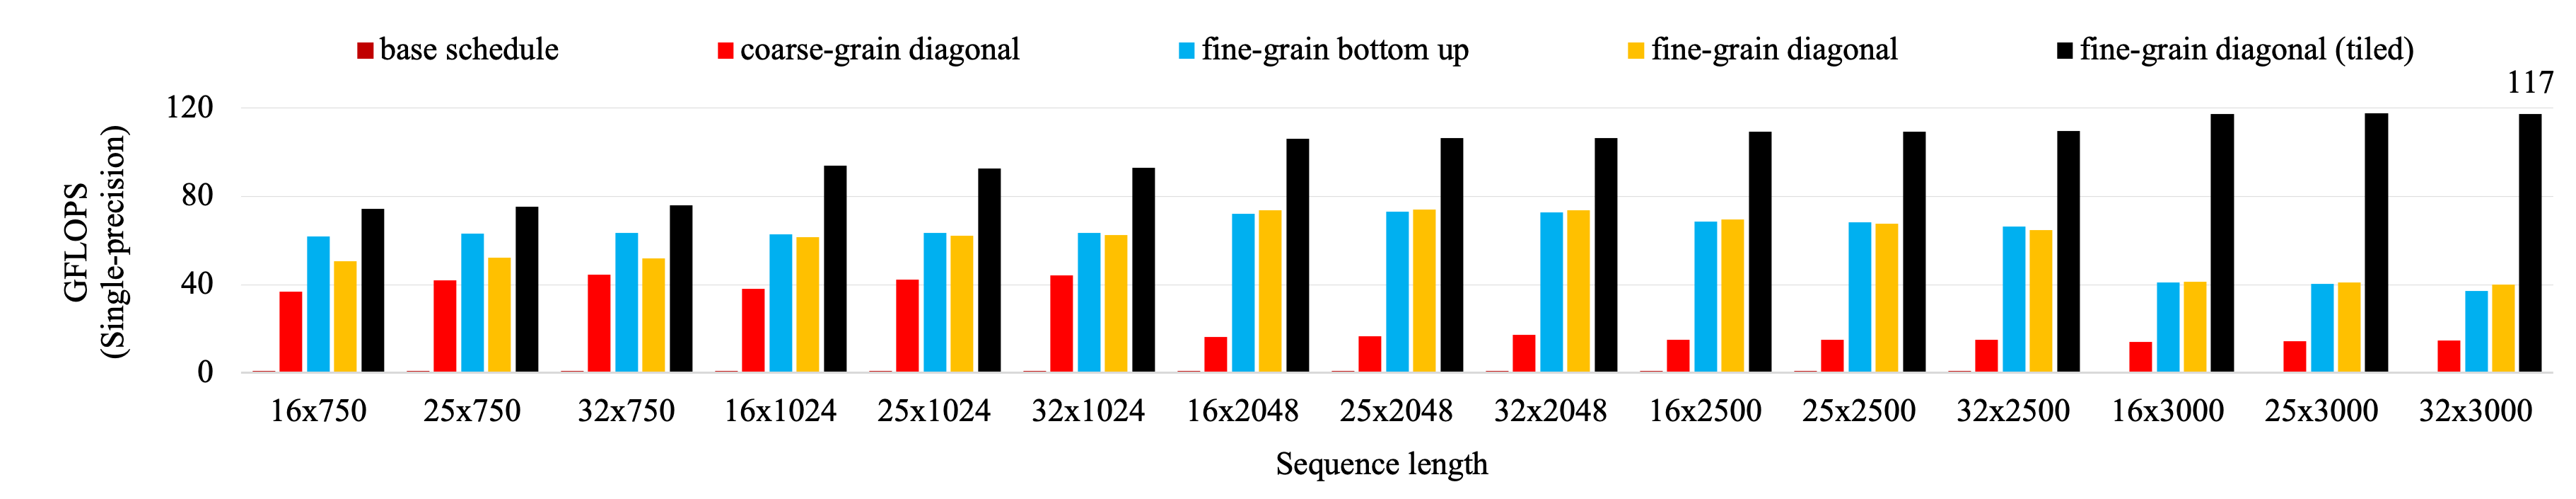
\includegraphics[width=\textwidth,scale=1.00, trim=5 5 5 5,clip]{dmp_performance_new.png}}
\caption{Double max-plus performance comparison}
\label{fig:peroformance_analysis_double_max_plus}
\end{figure*}

\begin{figure*}[htbp]
 \centerline{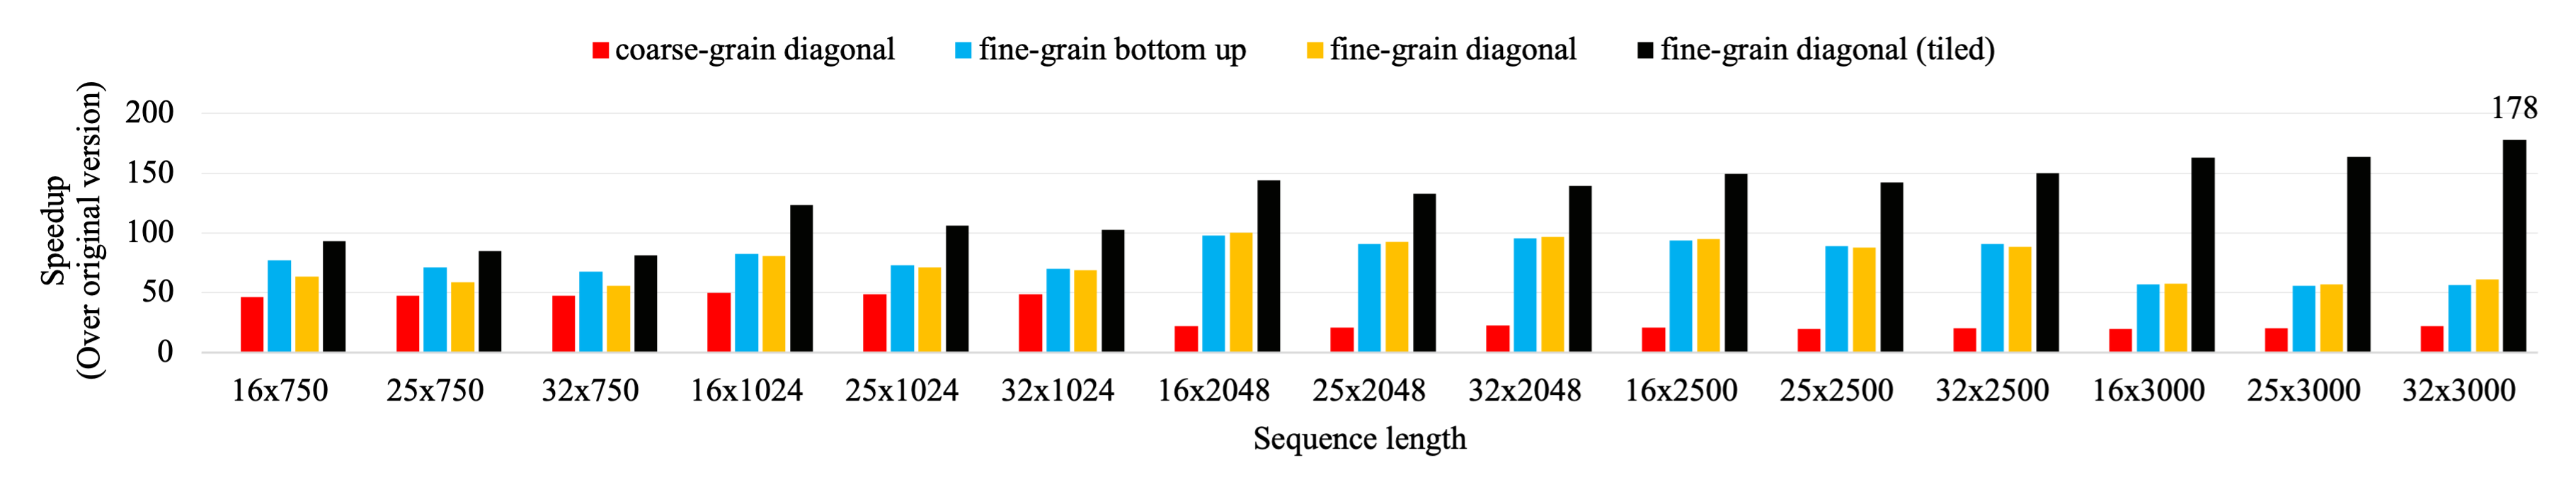
\includegraphics[width=\textwidth,scale=1.00, trim=5 5 5 5,clip]{dpm_speed_up_new.png}} 
%\end{adjustbox}
\caption{Double max-plus speedup comparison}
\label{fig:double_max_plus_speed_up}
\end{figure*}


\begin{figure*}[htbp]
\centerline{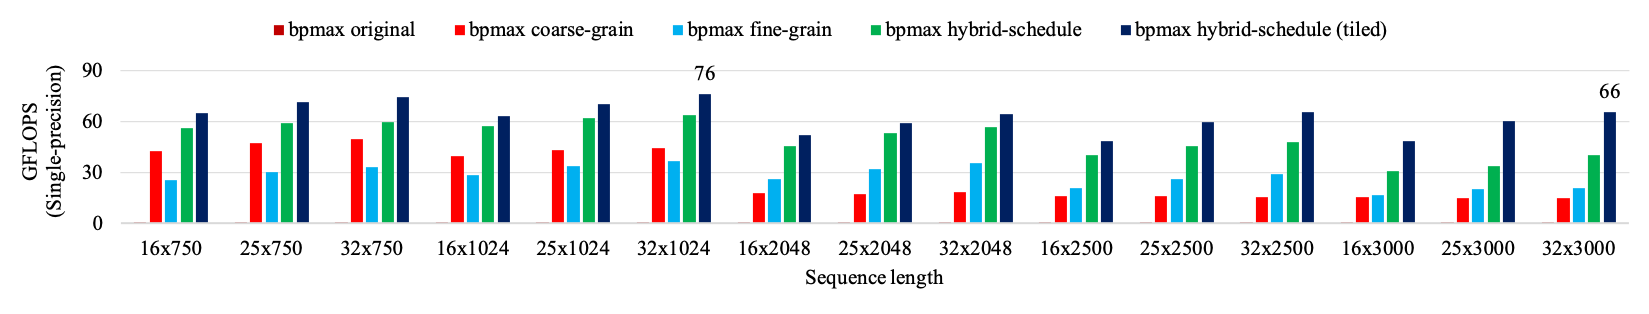
\includegraphics[width=\textwidth,scale=1.00, trim=5 5 5 5,clip]{bpm_performance_new.png}} 
\caption{BPMax performance comparison}
\label{fig:bpm_performance}
\end{figure*}

\begin{figure*}[htbp]
\centerline{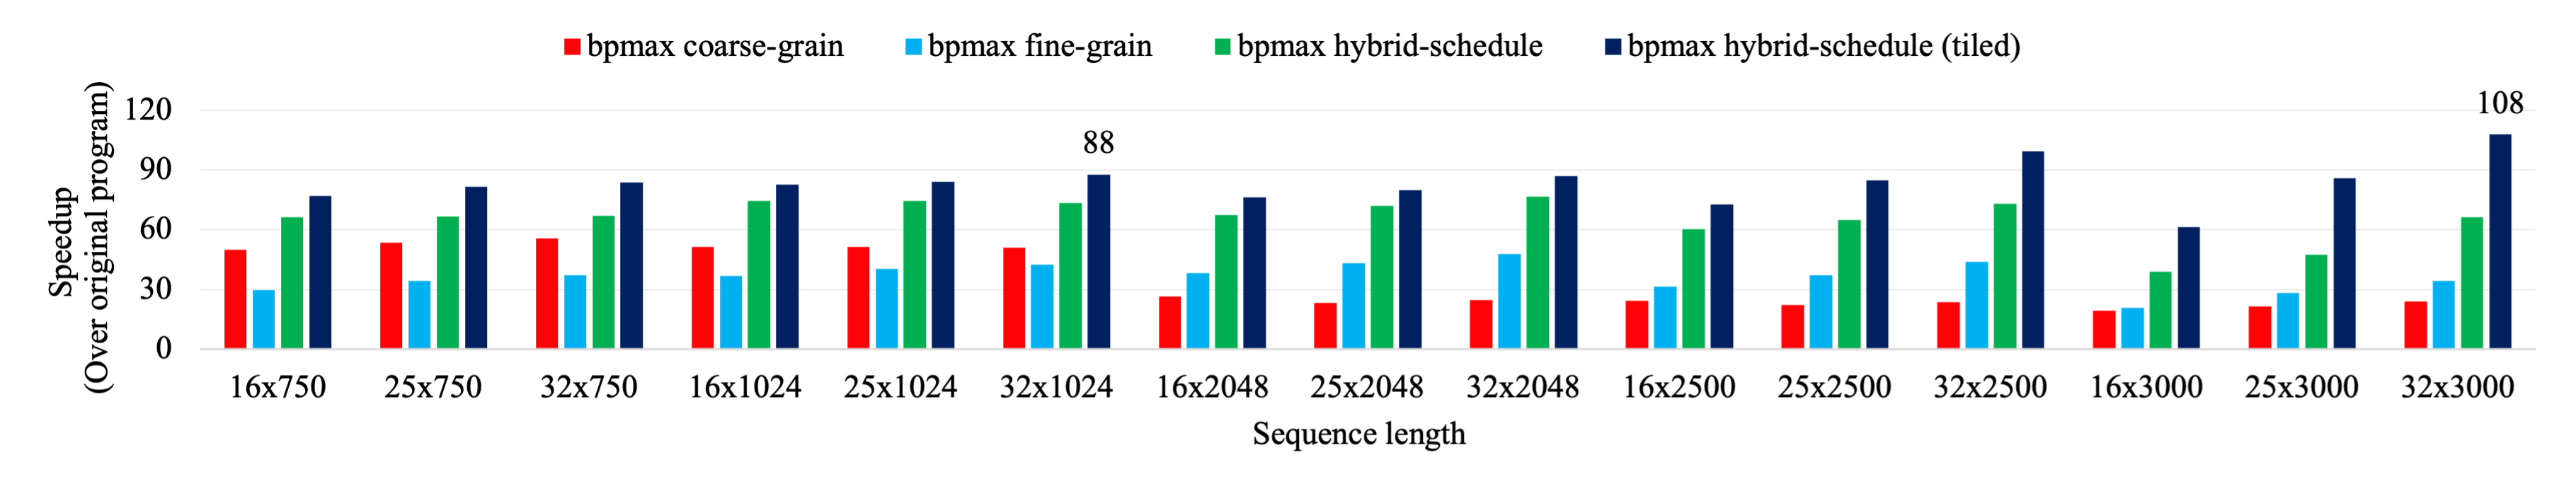
\includegraphics[width=\textwidth,scale=1.00, trim=5 5 5 5,clip]{bpm_speed_up_new.png}} 
\caption{BPMax speedup comparison}
\label{fig:bpm_speed_up}
\end{figure*}

%\begin{figure*}[!t]
%\centering
%\begin{subfigure}[t]{0.48\linewidth}
%\centering
%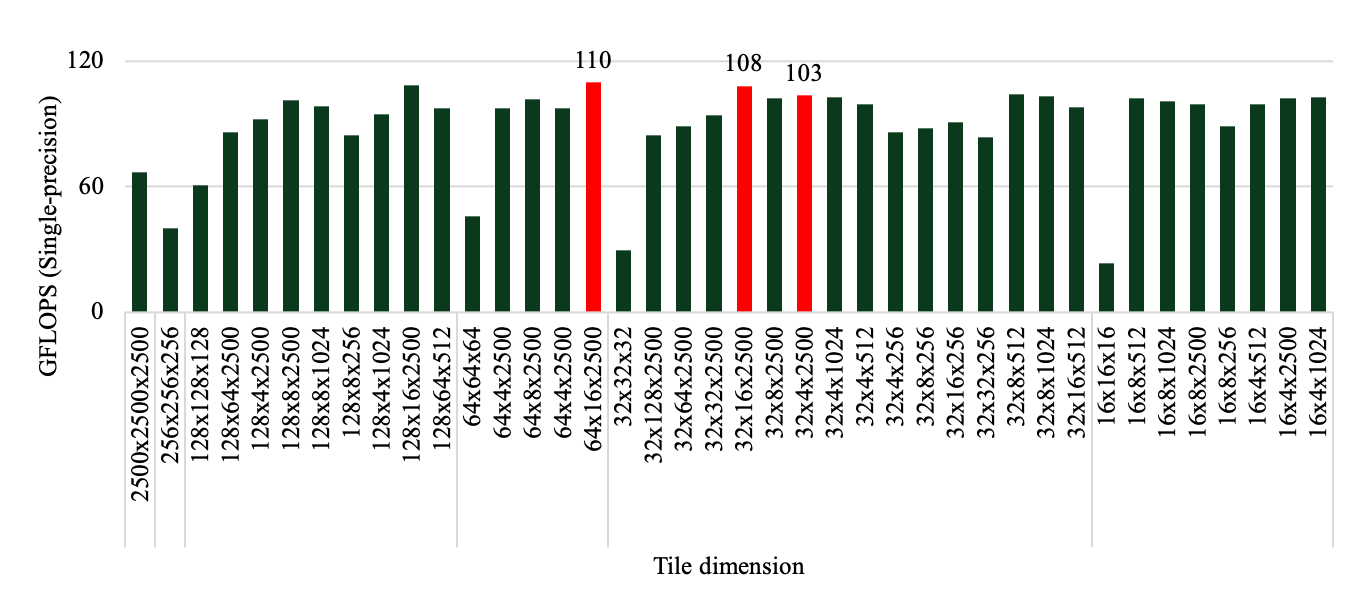
\includegraphics[scale=0.38, trim=5 5 5 5,clip]{double_max_plus_tile_exploration.png}
%\caption{Effect of tiling parameters ($i_{2} \times k_{2} \times j_{2}$) on double max-plus performance  - sequence length 16 x 2500}
%%\label{fig:tiling_parameter}
%\end{subfigure}
%\begin{subfigure}[t]{0.48\linewidth}
%\centering
%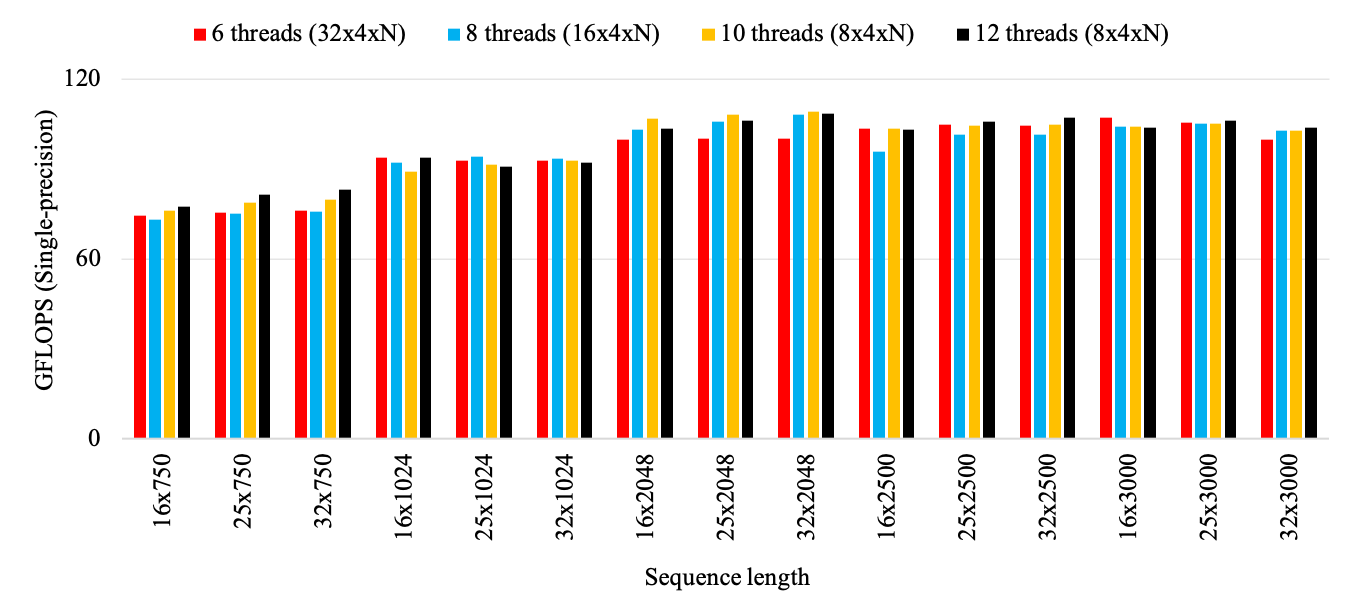
\includegraphics[scale=0.48, trim=5 5 5 5,clip]{double_max_plus_hyperthreading_new.png}
%\caption{Effect of hyper-threading on tiled double max-plus performance}
%\label{fig:hyperthreading_effect}
%\end{subfigure}
%\end{figure*}

\begin{figure}[htbp]
\centerline{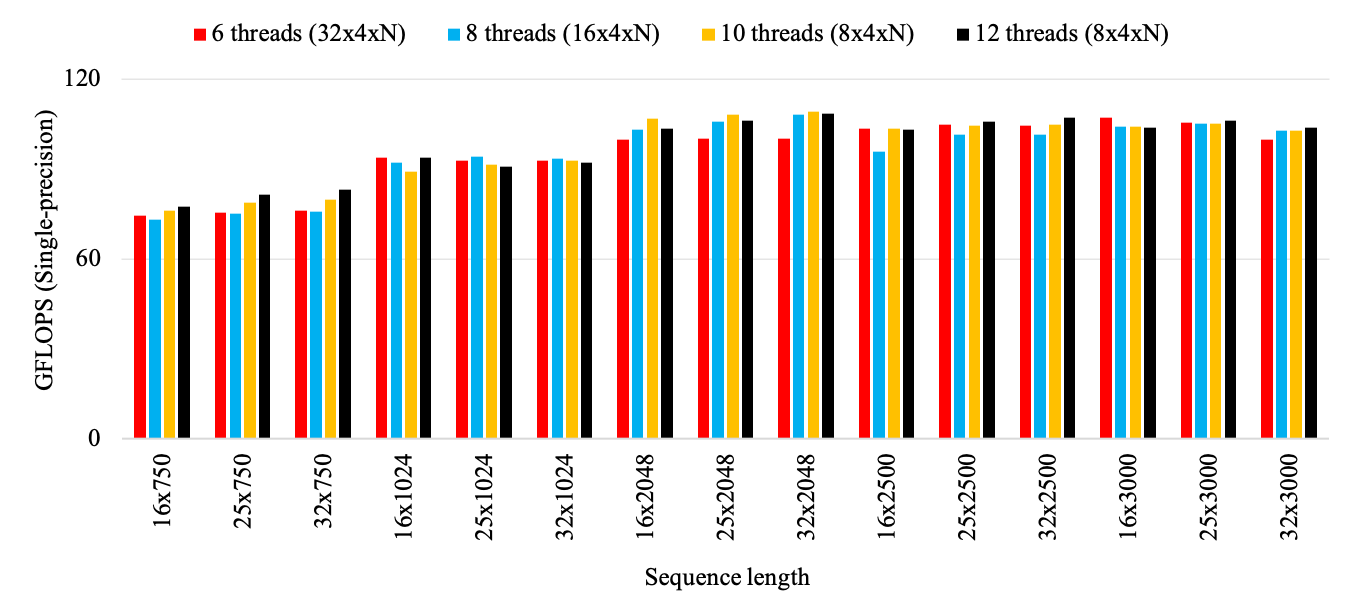
\includegraphics[scale=0.40, trim=4 4 4 4,clip]{double_max_plus_hyperthreading_new.png}}
\caption{Effect of hyper-threading on tiled double max-plus performance}
\label{fig:hyperthreading_effect}
\end{figure}

\begin{figure}[htbp]
\centerline{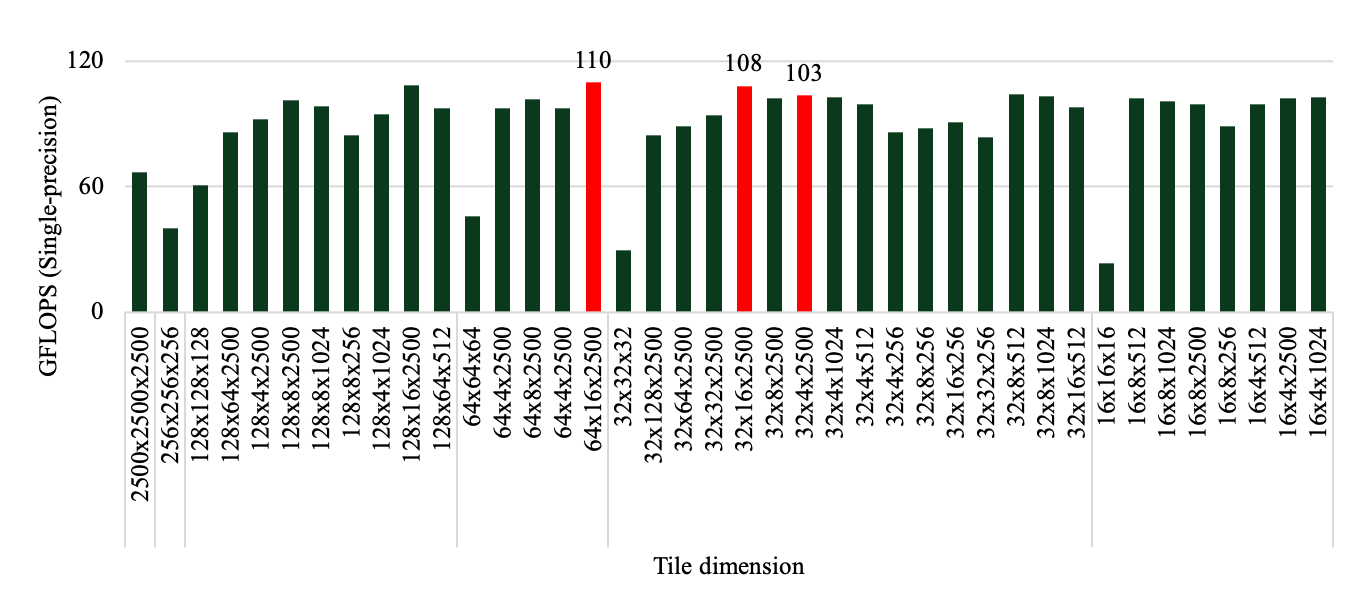
\includegraphics[scale=0.40, trim=4 4 4 4,clip]{double_max_plus_tile_exploration.png}}
\caption{Effect of tiling parameters ($i_{2} \times k_{2} \times j_{2}$) on double max-plus performance (sequence length - 16 x 2500)}
\label{fig:tiling_parameter}
\end{figure}


\subsection{BPMax  Performance Improvement}
Figure~\ref{fig:bpm_performance} and ~\ref{fig:bpm_speed_up} show the performance improvements and speedup  of different versions of the BPMax program using $6$ threads. We use the original BPMax program as the reference since no better CPU-version of the BPMax program is available. The coarse and fine-grain version of the program performs the worst, highlighted in light red and blue. As seen in the previous section, the coarse-grain schedule severely impacts double max-plus computation, affecting overall performance. Fine-grain parallelism works better for $R_0$, $R_3$, $R_4$, but we cannot parallelize the $R_1$, and $R_2$ computations. The hybrid parallelization approach highlighted in green performs better than the coarse and fine-grain schedule. The tiled version of the hybrid schedule highlighted in dark blue performs best. It achieves $100\times$ speedup for longer sequence lengths with $6$ threads. The improvement for the tiled version mainly comes from the optimization of $R_0$, $R_3$, $R_4$. The tiled version of the program reaches around $76$ GFLOPS for moderate-size sequences. It is almost $60\%$ lower than the best double max-plus version of the same sequence. Our analysis shows that $R_3$ and $R_4$ are almost free since those get computed along with the $R_0$. The other two $\Theta(M^2N^3)$ computations - $R_{1}$ and $R_{2}$ severely affect the overall performance. It is the effect of our schedule choice. Each thread is responsible for producing the final version of one inner triangle of $F$-table along with the $R_{1}$ and $R_{2}$. Both of these computations require most of the elements of one inner triangle of $F$-table and the $S^{(2)}$-table to compute one row for the worst case. So, the total amount of data required to process a row reaches about $\Theta(N^2)$, which is $16$ MB for an inner sequence of length $2048$. This issue gets amplified when we attempt hyper-threading (beyond $6$ threads for E5-1650v4).  

%Besides Xeon E5-1650v4, we have verified that the performance of the optimized BPMax scales up on Intel Xeon E-2278G, which has eight cores. Figure~\ref{fig:bpm_quick_compare} shows an overview of the performance and speedup comparison on Xeon E-2278G  and Xeon E5-1650v4.
%We have tried to adjust the degree of parallelism to smaller than the number of physical cores for  $R_{1}$ and $R_{2}$. 

Besides Xeon E5-1650v4, we have verified the scalability of our optimized program on Intel Xeon E-2278G, which has eight cores and runs almost at the same speed as E5-1650v4. The optimized BPMax performs the same or better on  E-2278G compare to E5-1650v4, reaching close to one-fourth of the theoretical single-precision machine peak. Figure~\ref{fig:bpm_quick_compare} shows an overview of the performance and speedup comparison on Xeon E-2278G  and Xeon E5-1650v4.

\subsection{Code Generation Metric}

Table~\ref{tab1:codegen_metric} shows the line of code (\textit{LOC}) generated by \alphaz\ for different BPMax program versions. We see an increase in \textit{LOC}  when the program is optimized. Also, the table highlights the complexities (based on \textit{LOC}) between the double max-plus computation and the BPMax program.

\begin{table}[htbp]
\caption{\uppercase{Auto-generated code statistics}}
\begin{center}
\begin{tabular}{|c|c|c|c|}
\hline
\textbf{\textit{Implementation}}& {\textit{LOC}} & \textbf{\textit{${\mathrm{a}}$}} & \textbf{\textit{${\mathrm{b}}$}} \\
\hline
BPMax base  & 140 & 140 & NA   \\
\hline
Double max-plus(coarse/fine)  & 150 & None & 3   \\
\hline
BPMax coarse/fine/ hybrid & 1200 & None & 30  \\
\hline
BPMax hybrid with tiled & 1400 & $<$5 & 7   \\
\hline
\multicolumn{3}{l}{${\mathrm{a}}$ - Hand written code}\\
\multicolumn{3}{l}{${\mathrm{b}}$ - Macro replacement/Macro comment out}\\
\end{tabular}
\label{tab1:codegen_metric}
\end{center}
\end{table}



\section{\uppercase{CONCLUSION}}
This work demonstrates the optimization process of a complete RRI program using polyhedral transformations. Our result shows that the tiling improves the performance of the most dominant part of the computation. However, the inner reductions are still inefficient, which limits the overall performance improvement. Also, the double max-plus operation remains bandwidth-bound even after tiling transformation. This indicates that an additional level of tiling at the register level is required to make the program compute-bound and improve performance.  We also plan to apply tiling on $R_1$ and $R_2$ and distribute the computation over a cluster using  MPI. All these transformations remain a challenge for \alphaz\ , and we hope to overcome them in the future.


% trigger a \newpage just before the given reference
% number - used to balance the columns on the last page
% adjust value as needed - may need to be readjusted if
% the document is modified later
%\IEEEtriggeratref{8}
% The "triggered" command can be changed if desired:
%\IEEEtriggercmd{\enlargethispage{-5in}}

% references section

% can use a bibliography generated by BibTeX as a .bbl file
% BibTeX documentation can be easily obtained at:
% http://mirror.ctan.org/biblio/bibtex/contrib/doc/
% The IEEEtran BibTeX style support page is at:
% http://www.michaelshell.org/tex/ieeetran/bibtex/
%\bibliographystyle{IEEEtran}
% argument is your BibTeX string definitions and bibliography database(s)
%\bibliography{IEEEabrv,../bib/paper}
%
% <OR> manually copy in the resultant .bbl file
% set second argument of \begin to the number of references
% (used to reserve space for the reference number labels box)


%\newpage
\bibliographystyle{IEEEtran}
\bibliography{biblio}
\end{document}
